\documentclass{article} % For LaTeX2e
\usepackage{graphicx}
\usepackage{caption}
\usepackage{subcaption}
\usepackage{amssymb}
\usepackage{amsmath}
\usepackage{nips14submit_e,times}
\usepackage{hyperref}
\usepackage{url}
\usepackage{verbatim}
%\usepackage{natbib}
%\documentstyle[nips14submit_09,times,art10]{article} % For LaTeX 2.09

\DeclareMathOperator{\x}{\mathbf{x}}
\DeclareMathOperator{\e}{\mathbf{e}}
\DeclareMathOperator{\M}{\mathbf{M}}
\DeclareMathOperator{\w}{\mathbf{w}}
\newcommand{\fix}{\marginpar{FIX}}
\newcommand{\new}{\marginpar{NEW}}
\edef\polishl{\l} 



\RequirePackage{latexsym}
\RequirePackage{amsmath}
\RequirePackage{amssymb} 
\RequirePackage{color} 
\RequirePackage{bm}
\RequirePackage{color}
\RequirePackage{picinpar}

%%%%%%%% Stock standard definitions %%%%%%%%%%%%%%%

\newcommand{\wbt}{\widetilde{\mathbf{w}}}
\DeclareMathOperator{\ab}{\mathbf{a}}
\DeclareMathOperator{\abh}{\widehat{\ab}}
\DeclareMathOperator{\bb}{\mathbf{b}}
\DeclareMathOperator{\bbh}{\widehat{\bb}}
\DeclareMathOperator{\cb}{\mathbf{c}}
\DeclareMathOperator{\db}{\mathbf{d}}
\DeclareMathOperator{\eb}{\mathbf{e}}
\DeclareMathOperator{\fb}{\mathbf{f}}
\DeclareMathOperator{\gb}{\mathbf{g}}
\DeclareMathOperator{\hb}{\mathbf{h}}
\DeclareMathOperator{\ib}{\mathbf{i}}
\DeclareMathOperator{\jb}{\mathbf{j}}
\DeclareMathOperator{\kb}{\mathbf{k}}
\DeclareMathOperator{\lb}{\mathbf{l}}
\DeclareMathOperator{\mb}{\mathbf{m}}
\DeclareMathOperator{\nbb}{\mathbf{n}}
\DeclareMathOperator{\ob}{\mathbf{o}}
\DeclareMathOperator{\pb}{\mathbf{p}}
\DeclareMathOperator{\qb}{\mathbf{q}}
\DeclareMathOperator{\rb}{\mathbf{r}}
\DeclareMathOperator{\sbb}{\mathbf{s}}
\DeclareMathOperator{\tb}{\mathbf{t}}
\DeclareMathOperator{\ub}{\mathbf{u}}
\DeclareMathOperator{\vb}{\mathbf{v}}
\DeclareMathOperator{\wb}{\mathbf{w}}
\DeclareMathOperator{\xb}{\mathbf{x}}
\DeclareMathOperator{\yb}{\mathbf{y}}
\DeclareMathOperator{\zb}{\mathbf{z}}
\renewcommand{\l}{\ell}

\DeclareMathOperator{\atilde}{\tilde{\ab}}
\DeclareMathOperator{\btilde}{\tilde{\bb}}
\DeclareMathOperator{\ctilde}{\tilde{\cb}}
\DeclareMathOperator{\dtilde}{\tilde{\db}}
\DeclareMathOperator{\etilde}{\tilde{\eb}}
\DeclareMathOperator{\ftilde}{\tilde{\fb}}
\DeclareMathOperator{\gtilde}{\tilde{\gb}}
\DeclareMathOperator{\htilde}{\tilde{\hb}}
\DeclareMathOperator{\itilde}{\tilde{\ib}}
\DeclareMathOperator{\jtilde}{\tilde{\jb}}
\DeclareMathOperator{\ktilde}{\tilde{\kb}}
\DeclareMathOperator{\ltilde}{\tilde{\lb}}
\DeclareMathOperator{\mtilde}{\tilde{\mb}}
\DeclareMathOperator{\ntilde}{\tilde{\nbb}}
\DeclareMathOperator{\otilde}{\tilde{\ob}}
\DeclareMathOperator{\ptilde}{\tilde{\pb}}
\DeclareMathOperator{\qtilde}{\tilde{\qb}}
\DeclareMathOperator{\rtilde}{\tilde{\rb}}
\DeclareMathOperator{\stilde}{\tilde{\sbb}}
\DeclareMathOperator{\ttilde}{\tilde{\tb}}
\DeclareMathOperator{\utilde}{\tilde{\ub}}
\DeclareMathOperator{\vtilde}{\tilde{\vb}}
\DeclareMathOperator{\wtilde}{\tilde{\wb}}
\DeclareMathOperator{\xtilde}{\tilde{\xb}}
\DeclareMathOperator{\ytilde}{\tilde{\yb}}
\DeclareMathOperator{\ztilde}{\tilde{\zb}}

\DeclareMathOperator{\abar}{\bar{\ab}}
\DeclareMathOperator{\bbar}{\bar{\bb}}
\DeclareMathOperator{\cbar}{\bar{\cb}}
\DeclareMathOperator{\dbar}{\bar{\db}}
\DeclareMathOperator{\ebar}{\bar{\eb}}
\DeclareMathOperator{\fbar}{\bar{\fb}}
\DeclareMathOperator{\gbar}{\bar{\gb}}
\DeclareMathOperator{\hbbar}{\bar{\hb}}
\DeclareMathOperator{\ibar}{\bar{\ib}}
\DeclareMathOperator{\jbar}{\bar{\jb}}
\DeclareMathOperator{\kbar}{\bar{\kb}}
\DeclareMathOperator{\lbar}{\bar{\lb}}
\DeclareMathOperator{\mbar}{\bar{\mb}}
\DeclareMathOperator{\nbar}{\bar{\nbb}}
\DeclareMathOperator{\obar}{\bar{\ob}}
\DeclareMathOperator{\pbar}{\bar{\pb}}
\DeclareMathOperator{\qbar}{\bar{\qb}}
\DeclareMathOperator{\rbar}{\bar{\rb}}
\DeclareMathOperator{\sbar}{\bar{\sbb}}
\DeclareMathOperator{\tbar}{\bar{\tb}}
\DeclareMathOperator{\ubar}{\bar{\ub}}
\DeclareMathOperator{\vbar}{\bar{\vb}}
\DeclareMathOperator{\wbar}{\bar{\wb}}
\DeclareMathOperator{\xbar}{\bar{\xb}}
\DeclareMathOperator{\ybar}{\bar{\yb}}
\DeclareMathOperator{\zbar}{\bar{\zb}}

\DeclareMathOperator{\Ab}{\mathbf{A}}
\DeclareMathOperator{\Bb}{\mathbf{B}}
\DeclareMathOperator{\Cb}{\mathbf{C}}
\DeclareMathOperator{\Db}{\mathbf{D}}
\DeclareMathOperator{\Eb}{\mathbf{E}}
\DeclareMathOperator{\Fb}{\mathbf{F}}
\DeclareMathOperator{\Gb}{\mathbf{G}}
\DeclareMathOperator{\Hb}{\mathbf{H}}
\DeclareMathOperator{\Ib}{\mathbf{I}}
\DeclareMathOperator{\Jb}{\mathbf{J}}
\DeclareMathOperator{\Kb}{\mathbf{K}}
\DeclareMathOperator{\Lb}{\mathbf{L}}
\DeclareMathOperator{\Mb}{\mathbf{M}}
\DeclareMathOperator{\Nb}{\mathbf{N}}
\DeclareMathOperator{\Ob}{\mathbf{O}}
\DeclareMathOperator{\Pb}{\mathbf{P}}
\DeclareMathOperator{\Qb}{\mathbf{Q}}
\DeclareMathOperator{\Rb}{\mathbf{R}}
\DeclareMathOperator{\Sbb}{\mathbf{S}}
\DeclareMathOperator{\Tb}{\mathbf{T}}
\DeclareMathOperator{\Ub}{\mathbf{U}}
\DeclareMathOperator{\Vb}{\mathbf{V}}
\DeclareMathOperator{\Wb}{\mathbf{W}}
\DeclareMathOperator{\Xb}{\mathbf{X}}
\DeclareMathOperator{\Xbt}{\widetilde{\Xb}}
\DeclareMathOperator{\Xbh}{\widehat{\Xb}}
\DeclareMathOperator{\Xbs}{\widetilde{\Xb}}
\DeclareMathOperator{\Zbs}{\widetilde{\Zb}}
\DeclareMathOperator{\Kbs}{\widetilde{\Kb}}
\DeclareMathOperator{\Zbh}{\widehat{\Zb}}
\DeclareMathOperator{\Ubh}{\widehat{\Ub}}
\DeclareMathOperator{\Yb}{\mathbf{Y}}
\DeclareMathOperator{\Zb}{\mathbf{Z}}

\DeclareMathOperator{\Abar}{\bar{A}}
\DeclareMathOperator{\Bbar}{\bar{B}}
\DeclareMathOperator{\Cbar}{\bar{C}}
\DeclareMathOperator{\Dbar}{\bar{D}}
\DeclareMathOperator{\Ebar}{\bar{E}}
\DeclareMathOperator{\Fbar}{\bar{F}}
\DeclareMathOperator{\Gbar}{\bar{G}}
\DeclareMathOperator{\Hbar}{\bar{H}}
\DeclareMathOperator{\Ibar}{\bar{I}}
\DeclareMathOperator{\Jbar}{\bar{J}}
\DeclareMathOperator{\Kbar}{\bar{K}}
\DeclareMathOperator{\Lbar}{\bar{L}}
\DeclareMathOperator{\Mbar}{\bar{M}}
\DeclareMathOperator{\Nbar}{\bar{N}}
\DeclareMathOperator{\Obar}{\bar{O}}
\DeclareMathOperator{\Pbar}{\bar{P}}
\DeclareMathOperator{\Qbar}{\bar{Q}}
\DeclareMathOperator{\Rbar}{\bar{R}}
\DeclareMathOperator{\Sbar}{\bar{S}}
\DeclareMathOperator{\Tbar}{\bar{T}}
\DeclareMathOperator{\Ubar}{\bar{U}}
\DeclareMathOperator{\Vbar}{\bar{V}}
\DeclareMathOperator{\Wbar}{\bar{W}}
\DeclareMathOperator{\Xbar}{\bar{X}}
\DeclareMathOperator{\Ybar}{\bar{Y}}
\DeclareMathOperator{\Zbar}{\bar{Z}}

\DeclareMathOperator{\Abbar}{\bar{\Ab}}
\DeclareMathOperator{\Bbbar}{\bar{\Bb}}
\DeclareMathOperator{\Cbbar}{\bar{\Cb}}
\DeclareMathOperator{\Dbbar}{\bar{\Db}}
\DeclareMathOperator{\Ebbar}{\bar{\Eb}}
\DeclareMathOperator{\Fbbar}{\bar{\Fb}}
\DeclareMathOperator{\Gbbar}{\bar{\Gb}}
\DeclareMathOperator{\Hbbar}{\bar{\Hb}}
\DeclareMathOperator{\Ibbar}{\bar{\Ib}}
\DeclareMathOperator{\Jbbar}{\bar{\Jb}}
\DeclareMathOperator{\Kbbar}{\bar{\Kb}}
\DeclareMathOperator{\Lbbar}{\bar{\Lb}}
\DeclareMathOperator{\Mbbar}{\bar{\Mb}}
\DeclareMathOperator{\Nbbar}{\bar{\Nb}}
\DeclareMathOperator{\Obbar}{\bar{\Ob}}
\DeclareMathOperator{\Pbbar}{\bar{\Pb}}
\DeclareMathOperator{\Qbbar}{\bar{\Qb}}
\DeclareMathOperator{\Rbbar}{\bar{\Rb}}
\DeclareMathOperator{\Sbbar}{\bar{\Sb}}
\DeclareMathOperator{\Tbbar}{\bar{\Tb}}
\DeclareMathOperator{\Ubbar}{\bar{\Ub}}
\DeclareMathOperator{\Vbbar}{\bar{\Vb}}
\DeclareMathOperator{\Wbbar}{\bar{\Wb}}
\DeclareMathOperator{\Xbbar}{\bar{\Xb}}
\DeclareMathOperator{\Ybbar}{\bar{\Yb}}
\DeclareMathOperator{\Zbbar}{\bar{\Zb}}

\DeclareMathOperator{\Ahat}{\widehat{A}}
\DeclareMathOperator{\Bhat}{\widehat{B}}
\DeclareMathOperator{\Chat}{\widehat{C}}
\DeclareMathOperator{\Dhat}{\widehat{D}}
\DeclareMathOperator{\Ehat}{\widehat{E}}
\DeclareMathOperator{\Fhat}{\widehat{F}}
\DeclareMathOperator{\Ghat}{\widehat{G}}
\DeclareMathOperator{\Hhat}{\widehat{H}}
\DeclareMathOperator{\Ihat}{\widehat{I}}
\DeclareMathOperator{\Jhat}{\widehat{J}}
\DeclareMathOperator{\Khat}{\widehat{K}}
\DeclareMathOperator{\Lhat}{\widehat{L}}
\DeclareMathOperator{\Mhat}{\widehat{M}}
\DeclareMathOperator{\Nhat}{\widehat{N}}
\DeclareMathOperator{\Ohat}{\widehat{O}}
\DeclareMathOperator{\Phat}{\widehat{P}}
\DeclareMathOperator{\Qhat}{\widehat{Q}}
\DeclareMathOperator{\Rhat}{\widehat{R}}
\DeclareMathOperator{\Shat}{\widehat{S}}
\DeclareMathOperator{\That}{\widehat{T}}
\DeclareMathOperator{\Uhat}{\widehat{U}}
\DeclareMathOperator{\Vhat}{\widehat{V}}
\DeclareMathOperator{\What}{\widehat{W}}
\DeclareMathOperator{\Xhat}{\widehat{X}}
\DeclareMathOperator{\Yhat}{\widehat{Y}}
\DeclareMathOperator{\Zhat}{\widehat{Z}}

\DeclareMathOperator{\Abhat}{\widehat{\Ab}}
\DeclareMathOperator{\Bbhat}{\widehat{\Bb}}
\DeclareMathOperator{\Cbhat}{\widehat{\Cb}}
\DeclareMathOperator{\Dbhat}{\widehat{\Db}}
\DeclareMathOperator{\Ebhat}{\widehat{\Eb}}
\DeclareMathOperator{\Fbhat}{\widehat{\Fb}}
\DeclareMathOperator{\Gbhat}{\widehat{\Gb}}
\DeclareMathOperator{\Hbhat}{\widehat{\Hb}}
\DeclareMathOperator{\Ibhat}{\widehat{\Ib}}
\DeclareMathOperator{\Jbhat}{\widehat{\Jb}}
\DeclareMathOperator{\Kbhat}{\widehat{\Kb}}
\DeclareMathOperator{\Lbhat}{\widehat{\Lb}}
\DeclareMathOperator{\Mbhat}{\widehat{\Mb}}
\DeclareMathOperator{\Nbhat}{\widehat{\Nb}}
\DeclareMathOperator{\Obhat}{\widehat{\Ob}}
\DeclareMathOperator{\Pbhat}{\widehat{\Pb}}
\DeclareMathOperator{\Qbhat}{\widehat{\Qb}}
\DeclareMathOperator{\Rbhat}{\widehat{\Rb}}
\DeclareMathOperator{\Sbhat}{\widehat{\Sb}}
\DeclareMathOperator{\Tbhat}{\widehat{\Tb}}
\DeclareMathOperator{\Ubhat}{\widehat{\Ub}}
\DeclareMathOperator{\Vbhat}{\widehat{\Vb}}
\DeclareMathOperator{\Wbhat}{\widehat{\Wb}}
\DeclareMathOperator{\Xbhat}{\widehat{\Xb}}
\DeclareMathOperator{\Ybhat}{\widehat{\Yb}}
\DeclareMathOperator{\Zbhat}{\widehat{\Zb}}

\DeclareMathOperator{\Acal}{\mathcal{A}}
\DeclareMathOperator{\Bcal}{\mathcal{B}}
\DeclareMathOperator{\Ccal}{\mathcal{C}}
\DeclareMathOperator{\Dcal}{\mathcal{D}}
\DeclareMathOperator{\Ecal}{\mathcal{E}}
\DeclareMathOperator{\Fcal}{\mathcal{F}}
\DeclareMathOperator{\Gcal}{\mathcal{G}}
\DeclareMathOperator{\Hcal}{\mathcal{H}}
\DeclareMathOperator{\Ical}{\mathcal{I}}
\DeclareMathOperator{\Jcal}{\mathcal{J}}
\DeclareMathOperator{\Kcal}{\mathcal{K}}
\DeclareMathOperator{\Lcal}{\mathcal{L}}
\DeclareMathOperator{\Mcal}{\mathcal{M}}
\DeclareMathOperator{\Ncal}{\mathcal{N}}
\DeclareMathOperator{\Ocal}{\mathcal{O}}
\DeclareMathOperator{\Pcal}{\mathcal{P}}
\DeclareMathOperator{\Qcal}{\mathcal{Q}}
\DeclareMathOperator{\Rcal}{\mathcal{R}}
\DeclareMathOperator{\Scal}{\mathcal{S}}
\DeclareMathOperator{\Scalt}{\widetilde{\Scal}}
\DeclareMathOperator{\Tcal}{\mathcal{T}}
\DeclareMathOperator{\Ucal}{\mathcal{U}}
\DeclareMathOperator{\Vcal}{\mathcal{V}}
\DeclareMathOperator{\Wcal}{\mathcal{W}}
\DeclareMathOperator{\Xcal}{\mathcal{X}}
\DeclareMathOperator{\Ycal}{\mathcal{Y}}
\DeclareMathOperator{\Zcal}{\mathcal{Z}}

\DeclareMathOperator{\Atilde}{\widetilde{A}}
\DeclareMathOperator{\Btilde}{\widetilde{B}}
\DeclareMathOperator{\Ctilde}{\widetilde{C}}
\DeclareMathOperator{\Dtilde}{\widetilde{D}}
\DeclareMathOperator{\Etilde}{\widetilde{E}}
\DeclareMathOperator{\Ftilde}{\widetilde{F}}
\DeclareMathOperator{\Gtilde}{\widetilde{G}}
\DeclareMathOperator{\Htilde}{\widetilde{H}}
\DeclareMathOperator{\Itilde}{\widetilde{I}}
\DeclareMathOperator{\Jtilde}{\widetilde{J}}
\DeclareMathOperator{\Ktilde}{\widetilde{K}}
\DeclareMathOperator{\Ltilde}{\widetilde{L}}
\DeclareMathOperator{\Mtilde}{\widetilde{M}}
\DeclareMathOperator{\Ntilde}{\widetilde{N}}
\DeclareMathOperator{\Otilde}{\widetilde{O}}
\DeclareMathOperator{\Ptilde}{\widetilde{P}}
\DeclareMathOperator{\Qtilde}{\widetilde{Q}}
\DeclareMathOperator{\Rtilde}{\widetilde{R}}
\DeclareMathOperator{\Stilde}{\widetilde{S}}
\DeclareMathOperator{\Ttilde}{\widetilde{T}}
\DeclareMathOperator{\Utilde}{\widetilde{U}}
\DeclareMathOperator{\Vtilde}{\widetilde{V}}
\DeclareMathOperator{\Wtilde}{\widetilde{W}}
\DeclareMathOperator{\Xtilde}{\widetilde{X}}
\DeclareMathOperator{\Ytilde}{\widetilde{Y}}
\DeclareMathOperator{\Ztilde}{\widetilde{Z}}


%%%%%%%% Widely accepted definitions %%%%%%%%%%%%%%%

\DeclareMathOperator{\CC}{\mathbb{C}} % Complex numbers
\DeclareMathOperator{\EE}{\mathbb{E}} % Expectation
\DeclareMathOperator{\KK}{\mathbb{K}} % Arbitrary field
\DeclareMathOperator{\MM}{\mathbb{M}} % Median
\DeclareMathOperator{\NN}{\mathbb{N}} % Natural numbers
\DeclareMathOperator{\PP}{\mathbb{P}} % Probability
\DeclareMathOperator{\QQ}{\mathbb{Q}} % Rationals
\DeclareMathOperator{\RR}{\mathbb{R}} % Real numbers 
\DeclareMathOperator{\ZZ}{\mathbb{Z}} % Integers

\DeclareMathOperator{\one}{\mathbf{1}}  % Identity
\DeclareMathOperator{\zero}{\mathbf{0}} % Zero
\DeclareMathOperator{\TRUE}{\mathbf{TRUE}}  % True
\DeclareMathOperator{\FALSE}{\mathbf{FALSE}}  % False

\DeclareMathOperator*{\mini}{\mathop{\mathrm{minimize}}}
\DeclareMathOperator*{\maxi}{\mathop{\mathrm{maximize}}}
\DeclareMathOperator*{\argmin}{\mathop{\mathrm{argmin}}}
\DeclareMathOperator*{\argmax}{\mathop{\mathrm{argmax}}}
\DeclareMathOperator*{\argsup}{\mathop{\mathrm{argsup}}}
\DeclareMathOperator*{\arginf}{\mathop{\mathrm{arginf}}}
\DeclareMathOperator{\sgn}{\mathop{\mathrm{sign}}}
\DeclareMathOperator{\sign}{\mathop{\mathrm{sign}}}
\DeclareMathOperator{\tr}{\mathop{\mathrm{tr}}}
\DeclareMathOperator{\rank}{\mathop{\mathrm{rank}}}
\DeclareMathOperator{\traj}{\mathop{\mathrm{Traj}}}

%%%%%%%% Bold Greek Letters %%%%%%%%%%%%%%%
\DeclareMathOperator{\sigmab}{\bm{\sigma}}
\DeclareMathOperator{\Sigmab}{\mathbf{\Sigma}}


%%%%%%%% Mess around with LaTeX %%%%%%%%%%%%%%%

%% Some style files might actually define these variables.
%% So don't mess with them if they are already defined

\ifx\BlackBox\undefined
\newcommand{\BlackBox}{\rule{1.5ex}{1.5ex}}  % end of proof
\fi

\ifx\proof\undefined
\newenvironment{proof}{\par\noindent{\bf Proof\ }}{\hfill\BlackBox\\[2mm]}
% \else
% \renewenvironment{proof}{\par\noindent{\bf Proof\ }}{\hfill\BlackBox\\[2mm]}
\fi

%Trying to put all on Section track
%\makeatletter
%\@addtoreset{equation}{section}
%\def\theequation{\thesection.\arabic{equation}}
%\def\thetheorem{\thesection.\arabic{theorem}}
%\makeatother

%the below clashes with the previous defs of them... 
%in the style files
%\newtheorem{theorem}{Theorem}[section]
%\newtheorem{lemma}[theorem]{Lemma}
%\newtheorem{corollary}[theorem]{Corollary}
%\newtheorem{conjecture}[conjecture]{Conjecture}


%%%%%%%% Utility functions %%%%%%%%%%%%%%%

\newcommand{\eq}[1]{(\ref{#1})} 
\newcommand{\mymatrix}[2]{\left[\begin{array}{#1} #2 \end{array}\right]}
\newcommand{\mychoose}[2]{\left(\begin{array}{c} #1 \\ #2 \end{array}\right)}
\newcommand{\mydet}[1]{\det\left[ #1 \right]}
\newcommand{\sembrack}[1]{[\![#1]\!]}

\newcommand{\ea}{\emph{et al. }}
\newcommand{\eg}{\emph{e.g. }}
\newcommand{\ie}{\emph{i.e., }}

\newcommand{\mnote}[1]{\marginpar{#1}}
\newcommand{\note}[1]{{\bf {#1}}}

%%%%%%%% Specific symbols for this project %%%%%%%%%%%%%%%

\DeclareMathOperator{\half}{\frac{1}{2}}

\newcommand{\Ref}[1]{\hfill\Green{[#1]}}
\DeclareMathOperator{\XX}{\mathcal{X}}
\newcommand{\ar}{\implies}
\newcommand{\yh}{\hat{y}}
\DeclareMathOperator{\lan}{\langle}
\DeclareMathOperator{\ran}{\rangle}

\DeclareMathOperator{\dc}{\mathrm{dc}}

\DeclareMathOperator{\Utb}{\widetilde{\Ub}}
\DeclareMathOperator{\Stb}{\widetilde{\Sbb}}

\ifx\Brown\undefined
\definecolor{brown}{rgb}{0.5,0.1,0.1}
\newcommand{\Brown}[1]{\color{brown}{#1}\color{black}}
\fi

\ifx\Red\undefined
\definecolor{red}{rgb}{1.0,0,0}
\newcommand{\Red}[1]{\color{red}{#1}\color{black}}
\fi

\ifx\Green\undefined
\definecolor{green}{rgb}{0,0.4,0}
\newcommand{\Green}[1]{\color{green}{#1}\color{black}}
\fi

\ifx\Blue\undefined
\definecolor{blue}{rgb}{0,0,1.0}
\newcommand{\Blue}[1]{\color{blue}{#1}\color{black}}
\fi



\newcommand{\beq}{\begin{equation}}
\newcommand{\eeq}{\end{equation}}
\newcommand{\beh}{\begin{conjecture}}
\newcommand{\eeh}{\end{conjecture}}
\newcommand\bel{\begin{lemma}}
\newcommand\eel{\end{lemma}}
\newcommand\bet{\begin{theoreme}}
\newcommand\eet{\end{theoreme}}
\newcommand\bex{\begin{example}}
\newcommand\eex{\end{example}}
\newcommand\bed{\begin{definition}}
\newcommand\eed{\end{definition}}
\newcommand\bep{\begin{proposition}}
\newcommand\eep{\end{proposition}}
\newcommand\ber{\begin{remark}}
\newcommand\eer{\end{remark}}
\newcommand\bec{\begin{corollary}}
\newcommand\eec{\end{corollary}}
%\newcommand\proof{\noindent {\bf Proof.}\ \ }
\newcommand\qed{\hfill$\Box$\medskip}
\newcommand\cP{{\mathcal P}}
\newcommand\cJ{{\mathcal J}}
\newcommand\cD{{\mathcal D}}
\newcommand\cC{{\mathcal C}}
\newcommand\cO{{\mathcal O}}
\newcommand\cS{{\mathcal S}}
\newcommand\cT{{\mathcal T}}
\newcommand\cV{{\mathcal V}}
\newcommand\cW{{\mathcal W}}
\newcommand\cY{{\mathcal Y}}
\newcommand\cF{{\mathcal F}}
\newcommand\cU{{\mathcal U}}
\newcommand\cE{{\mathcal E}}
\newcommand\cG{{\mathcal G}}
\newcommand\cB{{\mathcal B}}
\newcommand\cI{{\rm I}}
\newcommand\cN{{\mathcal N}}
\newcommand\cM{{\mathcal M}}
\newcommand\cA{{\mathcal A}}
\newcommand\cQ{{\mathcal Q}}
\newcommand\cK{{\mathcal K}}
\newcommand\cZ{{\mathcal Z}}
\newcommand\CAP{{\rm cap}}
\newcommand\ENT{{\rm ent}}
\newcommand\gr{{\rm gr}}

\def\qq{{\mathbb Q}}
\def\ff{{\mathbb F}}
\def\rr{{\mathbb R}}
\def\zz{{\mathbb Z}}
\def\cc{{\mathbb C}}
\def\nn{{\mathbb N}}
\def\kk{{\mathbb K}}
\def\ee{{\mathbb E}}
\def\ww{{\mathbb W}}
\def\hh{{\mathbb H}}
\def\ss{{\mathbb S}}
\def\tt{{\mathbb T}}
\def\pp{{\mathbb P}}



\newtheorem{theoreme}{Theorem} %[section]
\newtheorem{proposition}[theoreme]{Proposition}
\newtheorem{lemma}[theoreme]{Lemma}
\newtheorem{definition}[theoreme]{Definition}
\newtheorem{corollary}[theoreme]{Corollary}
\newtheorem{remark}[theoreme]{Remark}
\newtheorem{example}[theoreme]{Example}
\newtheorem{examples}[theoreme]{Examples}
%\newtheorem{conjecture}[theoreme]{Conjecture}
\newtheorem{conjecture}{Conjecture}


\title{An Information Theoretic Approach to Quantifying Text Interestingness}


\author{
David S.~Hippocampus\thanks{ Use footnote for providing further information
about author (webpage, alternative address)---\emph{not} for acknowledging
funding agencies.} \\
Department of Computer Science\\
Cranberry-Lemon University\\
Pittsburgh, PA 15213 \\
\texttt{hippo@cs.cranberry-lemon.edu} \\
\And
Coauthor \\
Affiliation \\
Address \\
\texttt{email} \\
\AND
Coauthor \\
Affiliation \\
Address \\
\texttt{email} \\
\And
Coauthor \\
Affiliation \\
Address \\
\texttt{email} \\
\And
Coauthor \\
Affiliation \\
Address \\
\texttt{email} \\
(if needed)\\
}

% The \author macro works with any number of authors. There are two commands
% used to separate the names and addresses of multiple authors: \And and \AND.
%
% Using \And between authors leaves it to \LaTeX{} to determine where to break
% the lines. Using \AND forces a linebreak at that point. So, if \LaTeX{}
% puts 3 of 4 authors names on the first line, and the last on the second
% line, try using \AND instead of \And before the third author name.

%\newcommand{\fix}{\marginpar{FIX}}
%\newcommand{\new}{\marginpar{NEW}}

%\nipsfinalcopy % Uncomment for camera-ready version

\begin{document}


\maketitle

\begin{abstract}

We study the problem of automatic prediction of text interestingness and present an information theoretic approach for
quantifying it in terms of topic diversity. Our hypothesis is, in many text domains, often an interesting
concept is generated by mixing a diverse set of topics. Given a word distributional model, we present
an approach that leverages {\sl Jensen-Shannon} divergence for measuring text diversity and demonstrate how such a measure
correlates with text interestingness. We describe several different base-line algorithms and present results over two different
data sets: a collection of e-commerce products from {\sl eBay} , and a corpus of {\sl NSF} abstracts.
\end{abstract}


%%%%%%%%%%%%%%%%%%%%%%%%%%%%%%%%%%%%%%%%%%%%%%%%%%%%%%%%%%%%%
%%%%%%%%%%%%%%%%%%%%%%%%%%%%%%%%%%%%%%%%%%%%%%%%%%%%%%%%%%%%%
%%%%%%%%%%%%%%%%%%%%%%%%%%%%%%%%%%%%%%%%%%%%%%%%%%%%%%%%%%%%%

\section{Introduction}
\label{sec:introduction}

With the rapid growth of e-commerce, new products are increasingly populated into the market place on daily basis.  A larger subset of these products are 
categorized as daily needs or off-the-shelf products, while a much smaller subset can be attributed as {\em unique}, {\em creative}, {\em serendipitous }, or {\em interesting} (see Figure~\ref{fig:ebay-products}). This class of products often provoke an emotive response in users and create a more engaging experience for the them (e.g.,  {\em Pinterest}). Automatic discovery of this type of products is an important problem in e-commerce for creating an engaging experience for the users.  

\begin{comment}
With the rapid growth of E-Commerce, new products are increasingly populated into the market place on daily basis.  A larger subset of these products are 
categorized as daily needs or off-the-shelf products, while a much smaller subset can be attributed as {\em unique}, {\em creative}, {\em serendipitous }, {\em conversation starter}, or {\em interesting}. This class of products often provoke an emotive response in users and create a more engaging experience for the them (see {\sl Pinterest}\footnote{\url{www.pinterest.com}} for example).  
Identifying this class of products is an important problem in E-commerce in order to create an engaging experience for the users. 
This is further illustrated in Figure~\ref{fig:ebay-products} where it shows a collection of {\sl eBay} products selected from several gadget related categories. The top row (Figures~\ref{fig:standard-iphone-case}, \ref{fig:standard-speaker}, and \ref{fig:standard-speaker}) shows examples of
off-the-shelf products that one might often see at stores, online sites, etc. In contast, the bottom row
(Figures~\ref{fig:eyeshadow-iphone-case}, \ref{fig:zeppelin-speaker}, and \ref{fig:geeky-clock}) shows examples of the products
from similar categories which are more unique and have a more creative design, and hence more {\em interesting}. 

Quantifying interestingness is a challenging problem. First, the general notion of interestingness is not well defined.  Second, it is 
subjective; something that is interesting to someone may not be interesting to someone else. There has been considerable research on visual interestingness and aesthetic quality of images~\cite{Datta:2006:SAP:2129560.2129588,Ke:2006:DHF:1153170.1153495,IsolaParikhTorralbaOliva2011,dhar:2011,reinecke2013predicting,journals/pami/WeinshallZHKOABGNPHP12}. 
In text domain, researchers have studied some dimensions of this problem in terms of {\em humor identification}~\cite{Mihalcea:2005:MCL:1220575.1220642,Davidov:2010:SRS:1870568.1870582,Kiddon11,labutov-lipson:2012:ACL2012short}, {\em text aesthetics}~\cite{journals:tamd:Schmidhuber10,N13-1118,ganguly:2014}, and {\em document diversity}~\cite{bache:2013}. 
\end{comment}

Quantifying interestingness is a challenging problem. There has been considerable research on visual interestingness and aesthetic quality of images~\cite{Datta:2006:SAP:2129560.2129588,Ke:2006:DHF:1153170.1153495,IsolaParikhTorralbaOliva2011,dhar:2011,reinecke2013predicting,journals/pami/WeinshallZHKOABGNPHP12}. 
In text domain, researchers have studied different dimensions of this problem in terms of {\em humor identification}~\cite{Mihalcea:2005:MCL:1220575.1220642,Davidov:2010:SRS:1870568.1870582,Kiddon11,labutov-lipson:2012:ACL2012short}, {\em text aesthetics}~\cite{journals:tamd:Schmidhuber10,N13-1118,ganguly:2014}, and {\em document diversity}~\cite{bache:2013}.  In this paper we only focus on the text. Our hypothesis is, many interesting products often present diversity in the text describing them. In examples shown in \ref{fig:ebay-products}, we have highlighted words that offer the largest diversity in each case.
For example in Figure~\ref{fig:eyeshadow-iphone-case}, in the context of iPhone cases, one would expect less to observe topics that relate to make up and so forth. In this paper we introduce an information-theoretic approach for measuring topic diversity based on {\em Jensen-Shannon Information Diversity} and show how it correlates with text interestingness. The idea of quantigfying topic diversity in text has been previously studied by~\cite{bache:2013} for measuring text diversity. We show how our method differs from this approaches and present empirical results over two different data sets: a collection of e-commerce products from {\sl eBay} , and a corpus of {\sl NSF} abstracts. 

\begin{figure}
\label{fig:ebay-products}
        \centering
         \begin{subfigure}[b]{0.3\textwidth}
        	        \centering
                
\includegraphics[width=25mm]{figures/eyeshadow-iphone-case.jpg}
                \caption{\textcolor{red}{{\bf Eyeshadow}} Palettes for \textcolor{red}{{\bf iPhone}} 6 case}
                \label{fig:eyeshadow-iphone-case}
        \end{subfigure}
              ~ %add desired spacing between images, e. g. ~, \quad, \qquad, \hfill etc.
          %(or a blank line to force the subfigure onto a new line)
        \begin{subfigure}[b]{0.3\textwidth}
		 \centering
                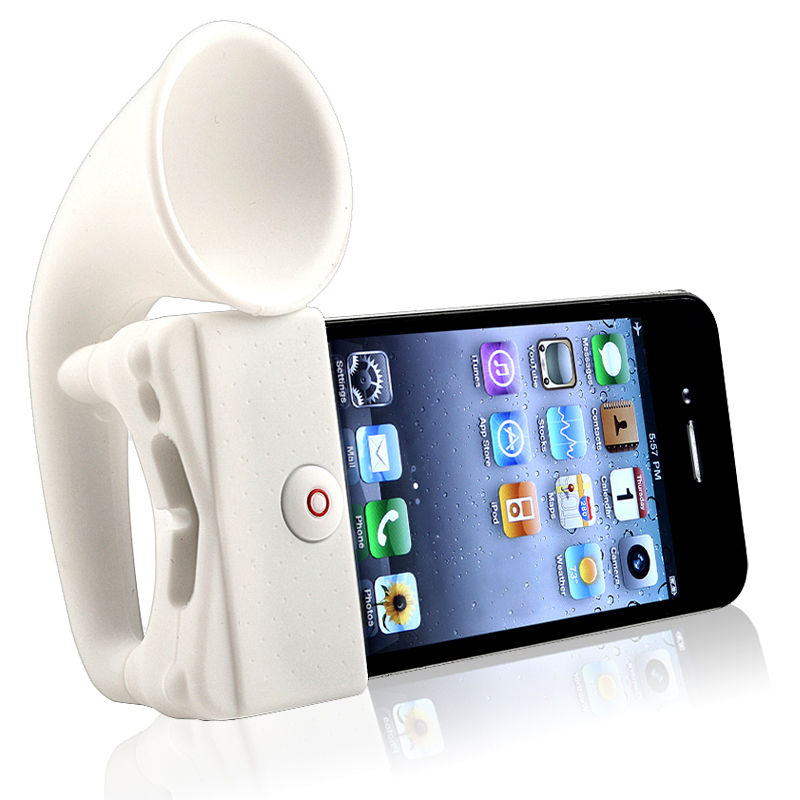
\includegraphics[width=25mm]{figures/horn-iphone-speaker.jpg}
\caption{White Silicone \textcolor{red}{{\bf Horn}} Stand Speaker for Apple \textcolor{red}{{\bf iPhone}} 4/ 4S}                \label{fig:zeppelin-speaker}
        \end{subfigure}
       ~ %add desired spacing between images, e. g. ~, \quad, \qquad, \hfill etc.
          %(or a blank line to force the subfigure onto a new line)
        \begin{subfigure}[b]{0.3\textwidth}
		 \centering
                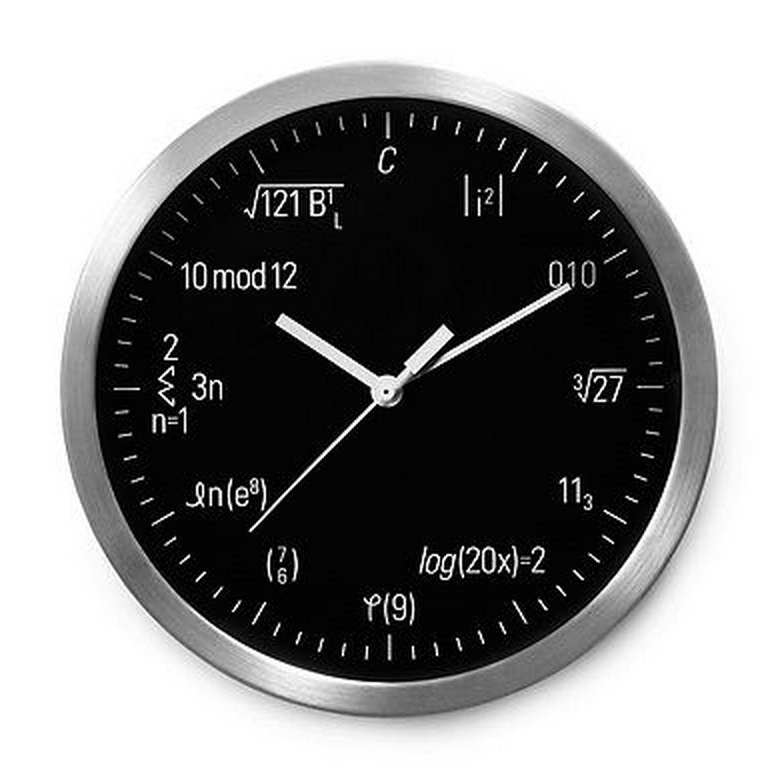
\includegraphics[width=30mm]{figures/geeky-clock.jpg}
\caption{\textcolor{red}{{\bf Equation}} Wall \textcolor{red}{{\bf Clock}} Gifts for Math Gurus}                \label{fig:geeky-clock}
        \end{subfigure}
       \caption{A collection of unique/interesting {\em eBay} products. Highlighted keywords demonstrate how the text associated with such products could span multiple diverse topics.}
       \label{fig:ebay-products}
\end{figure}

\begin{comment}
\begin{figure}
        \centering
        \begin{subfigure}[b]{0.3\textwidth}
                \centering
                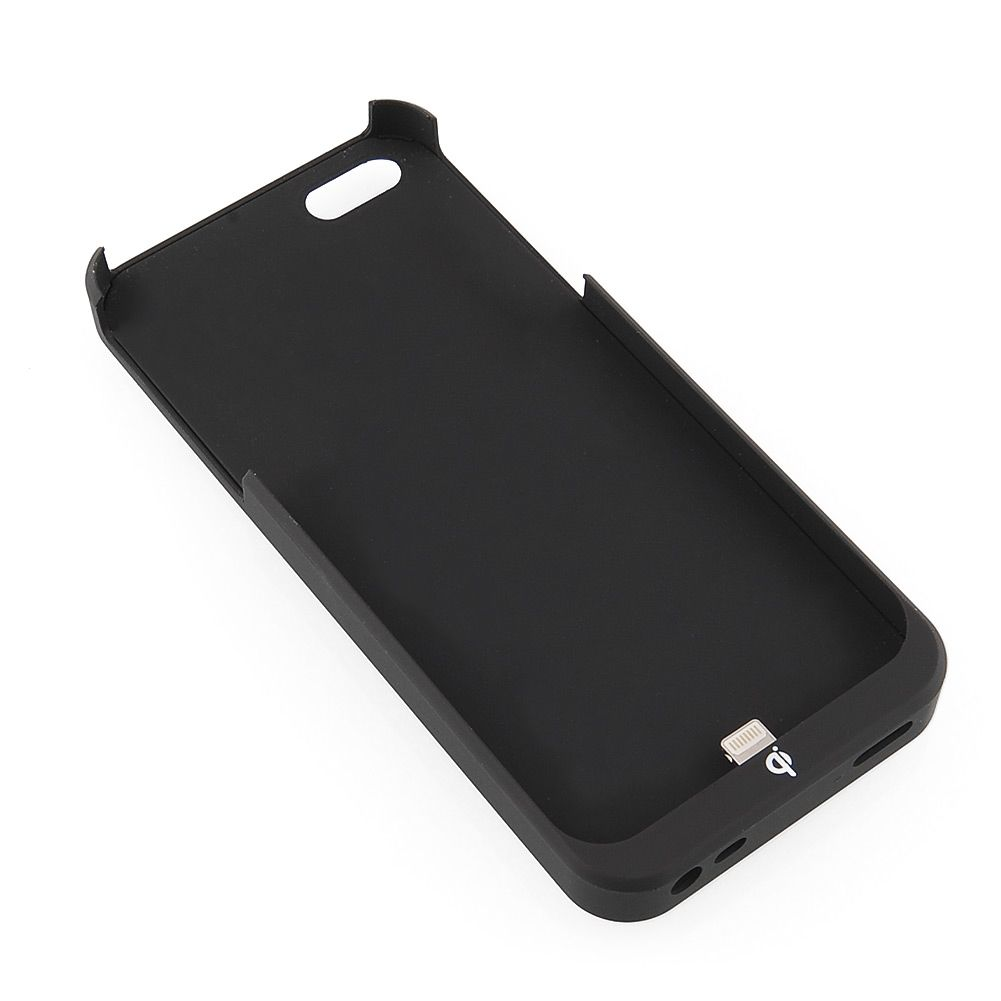
\includegraphics[width=25mm]{figures/standard-iphone-case.jpg}
                \caption{Black Qi Standard Wireless Charging Charger Receiver Case For iPhone 5 5G}
                \label{fig:standard-iphone-case}
        \end{subfigure}%
              ~ %add desired spacing between images, e. g. ~, \quad, \qquad, \hfill etc.
          %(or a blank line to force the subfigure onto a new line)
        \begin{subfigure}[b]{0.3\textwidth}
                \centering
                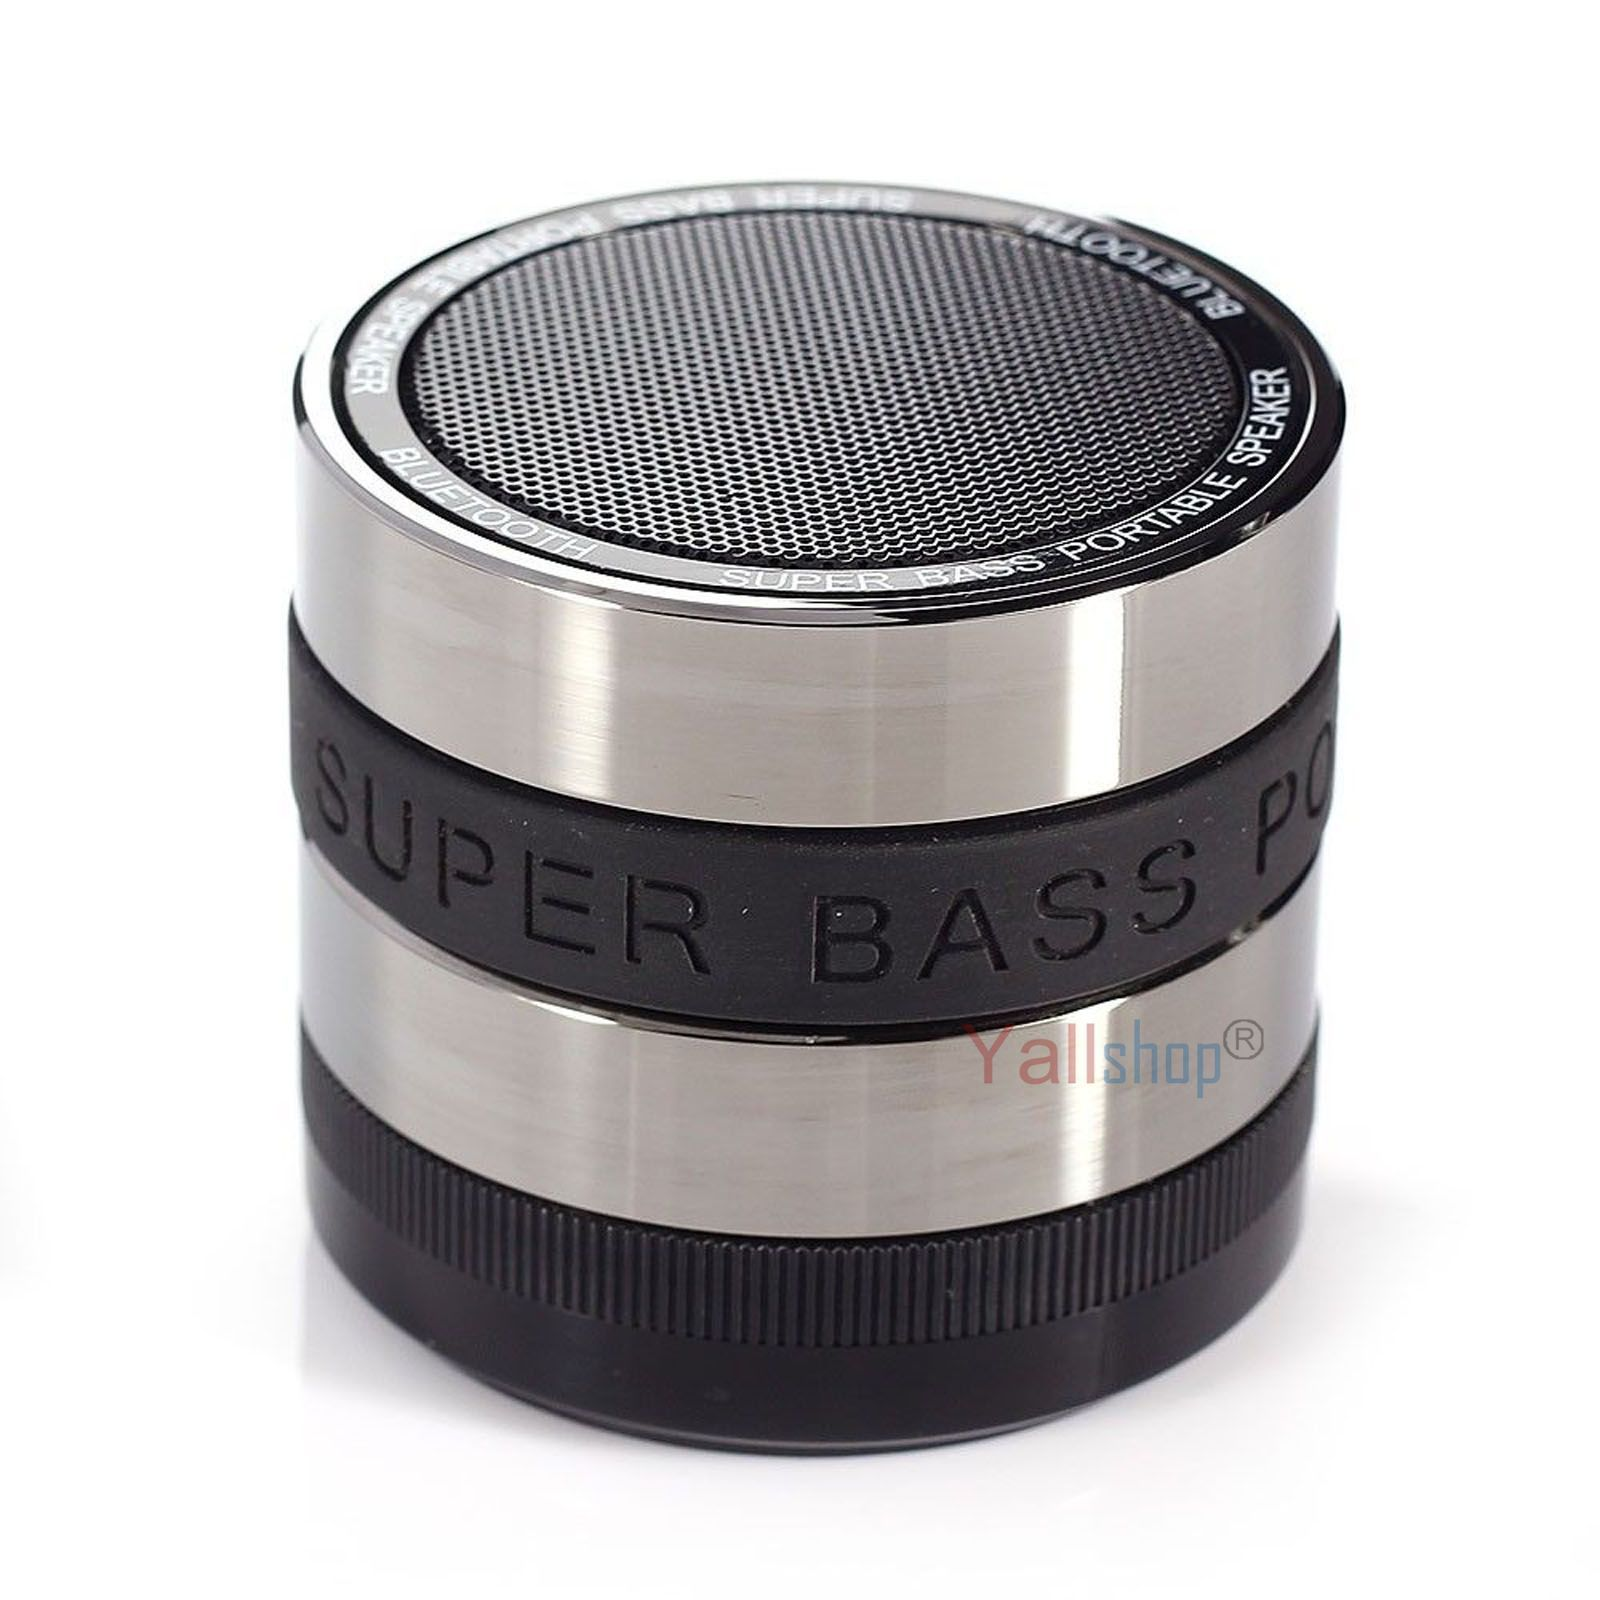
\includegraphics[width=25mm]{figures/standard-iphone-speaker.jpg}
                \caption{Bluetooth Wireless Speaker Mini Portable Super Bass For iPhone}
                \label{fig:standard-speaker}
        \end{subfigure}%
              ~ %add desired spacing between images, e. g. ~, \quad, \qquad, \hfill etc.
          %(or a blank line to force the subfigure onto a new line)
        \begin{subfigure}[b]{0.3\textwidth}
                \centering
                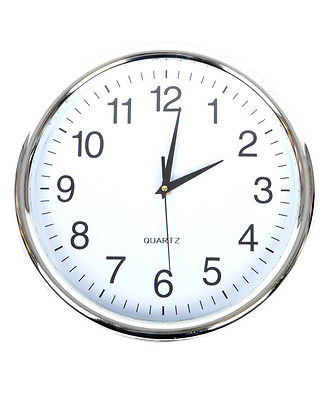
\includegraphics[width=25mm]{figures/standard-clock.jpg}
                \caption{Modern DIY Your Wall Clock Sticker Decoration Home Roman Numerals Silver SCY07}
                \label{fig:standard-speaker}
        \end{subfigure}\\
        ~ %add desired spacing between images, e. g. ~, \quad, \qquad, \hfill etc.
          %(or a blank line to force the subfigure onto a new line)
        \begin{subfigure}[b]{0.3\textwidth}
        	        \centering
                
\includegraphics[width=30mm]{figures/eyeshadow-iphone-case.jpg}
                \caption{\textcolor{red}{{\bf Eyeshadow}} Palettes for \textcolor{red}{{\bf iPhone}} 6 case}
                \label{fig:eyeshadow-iphone-case}
        \end{subfigure}
              ~ %add desired spacing between images, e. g. ~, \quad, \qquad, \hfill etc.
          %(or a blank line to force the subfigure onto a new line)
        \begin{subfigure}[b]{0.3\textwidth}
		 \centering
                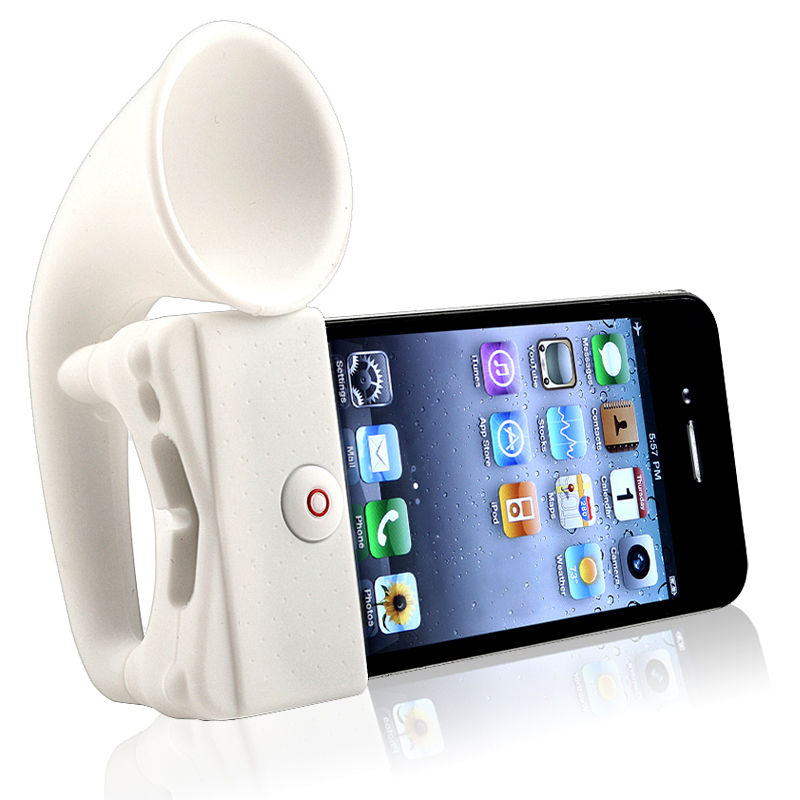
\includegraphics[width=30mm]{figures/horn-iphone-speaker.jpg}
\caption{White Silicone \textcolor{red}{{\bf Horn}} Stand Speaker for Apple \textcolor{red}{{\bf iPhone}} 4/ 4S}                \label{fig:zeppelin-speaker}
        \end{subfigure}
       ~ %add desired spacing between images, e. g. ~, \quad, \qquad, \hfill etc.
          %(or a blank line to force the subfigure onto a new line)
        \begin{subfigure}[b]{0.3\textwidth}
		 \centering
                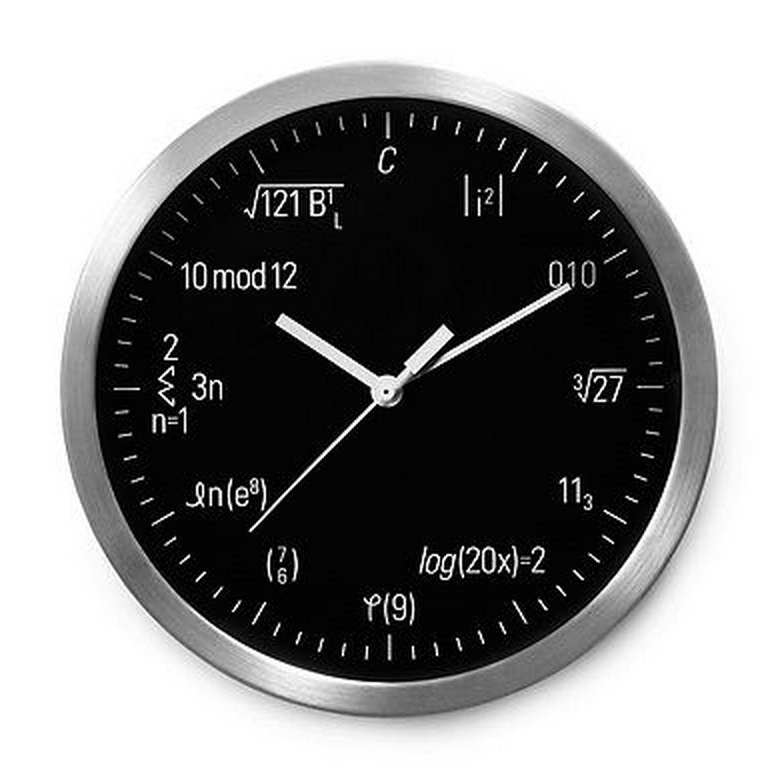
\includegraphics[width=30mm]{figures/geeky-clock}
\caption{\textcolor{red}{{\bf Equation}} Wall \textcolor{red}{{\bf Clock}} Gifts for Math Gurus or Best Geek Friends}                \label{fig:geeky-clock}
        \end{subfigure}
       \caption{A collection of {\em eBay} products: top row shows some off-the-shelf products while the bottom row shows a more unique/inteesting products of similar categories}\label{fig:ebay-products}
\end{figure}
\end{comment}






%% When looking at interestingness \cite{silva2006}















%%%%%%%%%%%%%%%%%%%%%%%%%%%%%%%%%%%%%%%%%%%%%%%%%%%%%%%%%%%%%
%%%%%%%%%%%%%%%%%%%%%%%%%%%%%%%%%%%%%%%%%%%%%%%%%%%%%%%%%%%%%
%%%%%%%%%%%%%%%%%%%%%%%%%%%%%%%%%%%%%%%%%%%%%%%%%%%%%%%%%%%%%

\section{Our Approach}
\label{sec:our-approach}

%\subsection{Word Representation}
%\label{sec:word-representation}

We assume a distributional representation for the words in the vocabulary (for a brief review
see~\cite{Turian10wordrepresentations}). A distributional representation over a vocabulary $V$ maps a word in the vocabulary to a 
probability distribution over a fixed set of contexts $C$. Often we start by a co-occurrence matrix $\cM_{|V|\times|C|}$ where each row represents a co-occurrence of a word with the set of contexts
$C$. For example if we chose $C=V$ then we obtain the familiar {\sl word-to-word} co-occurrence representation which counts the number
of times two words co-occurred in a document corpus. Another choice would be to use the set of topics learned over a document
corpus by {\sl Latent Dirichlet Allocation} (LDA)~\cite{Blei:2003:LDA:944919.944937} as the context. The rows of $A$
are then normalized in order to obtain a probability distribution over the context. We will use the notation $P_w$ to represent
the probability distribution over the context  given a word $w$. We also use the notation $T=\{w_1,...,w_k\}$ for a text
snippet where
$\{w_1,...,w_k\}$ are the words in the order they appear in the
text. Given a word distributional representation, $T_{\cP}=\{P_{w_1},...,P_{w_k}\}$ denotes the set of probability distributions over the words
in the text snippet.

%%%%%%%%%%%%%%%%%%%%%%%%%%%%%%%%%%%%%%%%%%%%%%%%%%%%%%%%%%%%%

\subsection{Information Diversity}
\label{sec:information-diversity}

Given a distributional representation over a vocabulary $W$ and context $C$ with $P_w$ giving a probability distribution of a
word $w$ over the context $C$, we can measure information diversity for a given text snippet $T=\{w_1,...,w_k\}$ and its
distributional representation $T_{\cP}=\{P_{w_1},...,P_{w_k}\}$ as follows:

\bed\label{importance}
Given a distribution $P_w$, its {\sl importance} with respect to a
prior distribution $P$ is defined as $D_w = D_{KL}(P_w\|P)$ where $D_{KL}(\|)$ denotes the
{\sl Kullback-Leibler} Divergence.
\eed

\bed\label{mixture}
Given a set of distributions $T_{\cP}=\{P_{w_1},...,P_{w_k}\}$ and a
prior $P$, we
define a mixture distribution $P_T$ as $P_T=\sum_{i=1}^k d_{w_i} P_{w_i}$ where $d_{w_i}=\frac{D_{w_i}}{\sum D_{w_j}}$ are the normalized
importances.
\eed

Essentially, $P_T$ is the weighted average of the set $T_{\cP}$, where
the weights are chosen according to the importances. Next we
define the diversity measure:

\bed\label{diversity}
We define the Jensen-Shannon Information Diversity of a set of
distributions $\cP_T$ with respect to 
prior $P$ as $D_S=\sum_{i=1}^k d_{w_i}D_{KL}(P_{w_i}\|P_T)$
where $d_{w_i}$ and $P_T$ are as in the previous definition.
\eed
This definition is closely related to the 
{\em general Jensen-Shannon Divergence}, defined in~\cite{FugledeTopsoe}. Another
interesting theoretical property of Jensen-Shannon Information
Diversity is that it can be interpreted as a generalization of Shannon
entropy as a population diversity measure, however we will not go
into this here any further. 

%%%%%%%%%%%%%%%%%%%%%%%%%%%%%%%%%%%%%%%%%%%%%%%%%%%%%%%%%%%%%

\subsection{Topic Diversity}
\label{sec:topic-diversity}

In order to apply this model to natural language we first need to build a distributional representation for words. One
natural choice for measuring the topic diversity is to use {\sl word-to-topic} distribution. We need to address the following problems:\\
{\bf (1) Building word to topic distribution}: We train an
LDA~\cite{Blei:2003:LDA:944919.944937} to build a topic model given a document corpus $\cC$. From this topic model we obtain the
word-topic matrix $\cM$ where $M_{ij}$ is the number of times $i$-th word was assigned the $j$-th topics . Note that word-topic distribution as described, is not directly defined in the standard {\em LDA} model and hence is only one possible approximation. By normalizing the rows of matrix $\cM$ we will obtain
a word-topic distribution, where the $i$-th row of the matrix gives the topic distribution for the word $w_i$.\\
{\bf (2) Obtaining a prior topic distribution} (which is
required for computing the information diversity as described in Section~\ref{sec:information-diversity}): We obtain a prior
 topic distribution by computing the proportions of overall topic
 assignments. This corresponds to summing up matrix $M$ along its
 columns (rows????), and then normalizing the resulting vector.\\
\begin{comment}
\begin{enumerate}
\item {\bf How to obtain a topic distribution for a given word}: We train an
LDA~\cite{Blei:2003:LDA:944919.944937} to build a topic model given a document corpus $\cC$. From this topic model we obtain the
word-topic matrix $\cM$ where $M_{ij}$ is the number of times $i$-th word was assigned the $j$-th topics\footnote{Note that word-topic distribution as described, is not directly defined in the standard {\em LDA} model and hence is only one possible approximation.}. By normalizing the rows of matrix $\cM$ we will obtain
a word-topic distribution, where the $i$-th row of the matrix gives the topic distribution for the word $w_i$.
\item {\bf How to obtain a prior topic distribution} (which is
required for computing the information diversity as described in Section~\ref{sec:information-diversity}): We obtain a prior
 topic distribution by computing the proportions of overall topic
 assignments. This corresponds to summing up matrix $M$ along its
 columns (rows????), and then normalizing the resulting vector.
\end{enumerate}
\end{comment}
%The proposed distributional model has some
%shortcomings\\
{\bf (3) Capturing topic similarity:} Here we consider the problem first raised in~\cite{bache:2013}. When building a word-to-topic distribution model based on 
the word-to-topic co-occurrence matrix, the relationship among topics may be lost (i.e, topic similarity ).  For example, if a word $w$
has a topic distribution $P_w$ concentrated on some topic $t$, then it will
not necessarily peek at all other topics that are very similar to topic $t$. To address this problem, we first define a topic similarity matrrix $\cS_{|T|\times|T|}$
where $i^{th}$ row of $\cS$ gives the topic similarity vector for the $i^{th}$ topic (e.g., {\em cosine} similarity between topics~\cite{bache:2013}). We further assume that it is normalized 
and hence can be thought of topic similarity a distribution. Using $\cS$ we obtain $\tilde{P}_w = P_w\cS^T$ which essentially diffuses the initial distribution to
one where  all topics similar to $t$ are well represented. Similarly, we can use $\cS$ to to reflect the topic similarity in the prior distribution as $\tilde{P} = P\cS^T$.
In Section~\ref{sec:experiments} we will show how this
approach enhances the standard entropic measure of diversity.\\
{\bf (4) Sample size bias problem:}  Note that 
when we normalize the rows of the matrix $\cM$ to obtain a distributional model, the normalization factor 
for every word is simply the word count. Thus for a word $w$ which occurs very rarely
in the entire corpus $\cC$, the topic distribution will be artificially skewed and is inaccurate simply because we do not have enough data points to estimate its true word-to-topic distribution.
Now, if for this corpus it happens that the prior topic distribution
is close to uniform, it will give a very high importance to the word
$w$ when measuring the information diversity as described in
Section~\ref{sec:information-diversity}.
One way to alleviate this
problem is to use the relative sample size (e.g., word count) to
smooth the distribution obtained by normalizing the rows of matrix
$\cM$. A natural choice for the smoothing distribution would in this
case be simply the prior distribution mentioned above. Applying {\em Laplace smoothing}
we get:
\begin{equation}
\widehat{P}_w=\frac{\alpha \tilde{P}+ \mu_w \tilde{P}_w}{\alpha+\mu_w}
\end{equation}
where $\mu_w$ is the frequency of word $w$ in D, and $P_w$ is the
topic assignment distribution obtained from the word-topic matrix,
while $\alpha$ is the parameter that specifies the strength of the
prior.\\
{\bf (5) Conditioning on context words:} We propose a final enhancement to the word-topic
distributions. Suppose, the set of words $T=\{w_1,...,w_k\}$
represents a text snippet that we want to analyze. The word $w_i$ has
a specific meaning inside of $T$, that can be significantly different
than its meaning out of context. We can describe that context using
the mixture distribution from Definition \ref{mixture}. Denote
$T_i=T-\{w_i\}$ as the set of all words in $T$ except
$w_i$. By $P_{T_i}$, we denote the mixture distribution for $T_i$. We
propose the following definition of context-dependent word-topic
distribution. 
\bed
Let $\widehat{P},\widehat{P}_{w_i},P_{T_i}$ be the topic prior, general
topic distribution for $w_i$, and the context distribution,
respectively. Then, the context-dependent distribution is
\begin{equation*}
P^{T_i}_{w_i}(t)\propto \frac{\tilde{P}_{T_i}(t)}{\tilde{P}(t)}\tilde{P}_{w_i}(t)
\end{equation*}
\eed
There is a probabilistic explanation that we have left out for 
lack of space. However this can be intuitively understood as follows:
we can think of $\frac{\tilde{P}_{T_i}(t)}{\tilde{P}(t)}$ as a weight
that further reshapes the smoothed word-to-topic distribution $\tilde{P}_{w_i}(t)$
to take into account the context. In our experiments we also smooth this distribution
using {\em Laplacian} smoothing.


\begin{comment}
Here we consider the issue first raised in \cite{bache:2013}, namely, that
when one tries to describe meaning through topic distribution, the
relations between the topics may be lost. For example, if a word $w$
has a topic distribution $P_w$ concentrated on one topic $t1$, then it will
not reflect the fact that $w$ is also closely related to $t2$ simply
because topics $t1$ and $t2$ are similar. Now, suppose that for each
topic $t$, we have a topic-similarity vector $S_t$ associated with
it. We will assume that it is normalized to a distribution and
represent those vectors as rows of a square matrix $S$. We propose
that instead of the distribution $P_w$, a more suited one would be
$P'_w=P_wS^T$. This can be derived probabilistically, but we can also look
at this as follows, for each topic $t$, instead of giving it
probability $P_w(t)$, we add to the final distribution the vector
$S_t$, scaled by $P_w(t)$. We expect that the topic $t$ itself has
high value for its index in $S_t(t)$, as do topics similar to
$t$. This way, a distribution $P_w$ concentrated on one topic $t$ would be
diffused to a distribution in which all topics similar to $t$ are well
represented. Notice, that this approach can be applied to any measure
of diversity based on a probability distribution, as long as we can
come up with a topic-similarity matrix $S$. We will show how this
approach enhances the standard entropic measure of diversity. This
approach is related to the one shown in [kevin], where a
topic-similarity matrix is also use, in a different way.
It remains to say how we obtain the topic-similarity vectors $S_t$. We
chose to use Cosine Similarity between topic word-vectors, as described in
[kevin]. \\
\end{coment}




\begin{comment}
The proposed distributional model based on the topic model has some
shortcomings. First, consider a word $w$ which occurs very rarely
in the entire corpus $\cC$. The word-to-topic distribution $P_w$ associated with this word
will be very concentrated. If for this corpus it happens that the prior topic distribution 
is close to uniform, it will give a very high importance to the word $w$, just because
there is not enough data points to determine its {\em true} topic distribution. 
\end{comment}

\begin{comment}
We will now present a model of a human Observer $A$ that is being presented with
the set $\cT$ and is supposed to judge the {\em interestingness} of
each piece of text from it. Additionally, we assume that $A$ has
gained their linguistic knowledge by observing samples from the set
$\cD$. What is, then, the general meaning (topic distribution) of a word $w$,
from the Observer's viewpoint? A statistically adequate approach is to
take a Bayesian model with a Dirichlet prior. We observe occurrences
in set $\cD$ of topic assignments for $w$ to learn the posterior
distribution. However, instead of using the fixed assignments produced
by the topic model, we let the Observer choose their own assignment as
follows: given a pair $(w,t)$, where $t$ is the topic assignment given
by the model for a specific occurrence of $w$, the observer selects a
topic from some topic-similarity distribution $S_t$, conditional on
$t$. An appropriate Dirichlet prior can be derived from this by
looking at the overall topic assignments (not for a specific
word). What would we get if we fed those to the Observer, letting $A$
generate their own topic for each?  Denoting by $S$ the matrix with
rows of topic-similarity distributions and by $P$ the (row vector) topic
distribution coming from the word-topic matrix, we find that the
observer's prior will concentrate around the distribution described by
the product $\widehat{P}=PS^T$. Using Bayes's rule to calculate the Observer's
posterior probability, we get
\[\widehat{P}_w=\frac{\alpha PS^T + \mu_w P_wS^T}{\alpha+\mu_w},\]
where $\mu_w$ is the frequency of word $w$ in D, and $P_w$ is the
topic assignment distribution obtained from the word-topic matrix,
while $\alpha$ is the parameter that specifies the strength of the
prior.
\end{comment}

\begin{comment}
Finally, we propose a third enhancement to the word-topic
distributions. Suppose, the set of words $T=\{w_1,...,w_k\}$
represents a text snippet that we want to analyze. The word $w_i$ has
a specific meaning inside of $T$, that can be significantly different
than its meaning out of context. We can describe that context using
the mixture distribution from Definition \ref{mixture}. Denote
$T_i=T-\{w_i\}$ as the set of all words in $T$ except
$w_i$. By $P_{T_i}$, we denote the mixture distribution for $T_i$. We
propose the following definition of context-dependent word-topic
distribution. 
\bed
Let $\widehat{P},\widehat{P}_{w_i},P_{T_i}$ be the topic prior, general
topic distribution for $w_i$, and the context distribution,
respectively. Then, the context-dependent distribution is
\[P^{T_i}_{w_i}(t)\propto \frac{\widehat{P}_{w_i}\!(t)P_{T_i}\!(t)}{\widehat{P}(t)}.\]
\eed
Without getting into the probabilistic explanation, we can roughly say
that context distribution $P_{T_i}$ reshapes $w_i$'s topic
distribution, putting most importance on those topics that have high
probabilties in both $P_{T_i}$ and in $\widehat{P}_{w_i}$.
The danger with relying on $P^{T_1}_{w_1}$
is that if the distributions $\widehat{P}_{w_1}$ and $P_{T_1}$ are
mostly disjoint, than their product will be very small. In other
words, we would need a long sampling process in generating the
hypothetical word-topic count matrix to obtain a statistically
significant estimation of the $P^{T_1}_{w_1}$. Once again,
we use Bayesian smoothing, with Dirichlet prior concentrated around
$\widehat{P}_{w_1}$, obtaining (with
parameter $\beta$ describing the strength of the prior):
\[\widehat{P}^{T_1}_{w_1}(t)\propto \beta \widehat{P}_{w_1}\!(t) + \frac{\widehat{P}_{w_1}\!(t)P_{T_1}\!(t)}{\widehat{P}(t)}.\]
\end{comment}

\begin{comment}
Next, let us analyze the Observer's behavior when reading a text
segment from $\cT$. We treat each piece of text as a bag of words,
disregarding the order. Suppose, the set of words is $T=\{w_1,...,w_k\}$. We
have already established how the Observer understands each word
separately. However, given a set of words, each one exists in the
context of the others. We can describe that context using the mixture
distribution from Definition \ref{mixture}. Denote
$T_1=\{w_2,...,w_k\}$ as the set of all words in $T$ except
$w_1$. What is the appropriate topic distribution for $w_1$, given a
context mixture distribution $P_{T_1}$? For this, we can look more
closely at the LDA model we used to obtain the word-topic matrix. We
can think of it as being generated by the following process: first
drawing a topic form the prior topic distribution, then drawing a word
from that topic's word distribution. It is natural to ask what would
the matrix look like if we used $P_{T_1}$ as the topic distribution
instead of the prior, and what would be the corresponding topic
distribution for word $w_1$. 

\bep
Let $\widehat{P},\widehat{P}_{w_1},P_{T_1}$ be the topic prior, general
topic distribution for $w_1$, and the context distribution,
respectively. Then, the context dependent distribution defined as
above, will be
\[P^{T_1}_{w_1}(t)\propto \frac{\widehat{P}_{w_1}\!(t)P_{T_1}\!(t)}{\widehat{P}(t)}.\]
\eep

The danger with relying on $P^{T_1}_{w_1}$
is that if the distributions $\widehat{P}_{w_1}$ and $P_{T_1}$ are
mostly disjoint, than their product will be very small. In other
words, we would need a long sampling process in generating the
hypothetical word-topic count matrix to obtain a statistically
significant estimation of the $P^{T_1}_{w_1}$. Once again,
we turn to bayesian analysis: we let the Observer use
$\widehat{P}_{w_1}$ as their maximum likelihood estimator in a
Dirichlet prior, obtaining the following posterior solution:
\[\widehat{P}^{T_1}_{w_1}(t)\propto \beta \widehat{P}_{w_1}\!(t) + \frac{\widehat{P}_{w_1}\!(t)P_{T_1}\!(t)}{\widehat{P}(t)}.\]
\end{comment}


%%%%%%%%%%%%%%%%%%%%%%%%%%%%%%%%%%%%%%%%%%%%%%%%%%%%%%%%%%%%%
%%%%%%%%%%%%%%%%%%%%%%%%%%%%%%%%%%%%%%%%%%%%%%%%%%%%%%%%%%%%%
%%%%%%%%%%%%%%%%%%%%%%%%%%%%%%%%%%%%%%%%%%%%%%%%%%%%%%%%%%%%%

\section{Experiments}
\label{sec:experiments}

We used the following two datasets in our experiments: (1) Interesting iPhone cases:
for generating the ground truth data we hired workers from {\em Amazon Mechanical Turk (AMT)} to label a collection
of nearly 20,000 iPhone cases on {\em eBay}. The details of this step is beyond the scope of this paper, however we used insights from
interesting iPhone cases found on {\em Pinterest} and {\em eBay's} user behavior data in order to generate a balanced data-set. 
We then pulled our final dataset from the annotated by selecting only those instances where the annotators all labeled it as
positive (i.e., interesting) or negative (i.e., uninteresting). The final data-set consists of 2179 positive and 9770 negative instances for
a total of 11,949 instances. For each instance, the product title of
the corresponding {\em eBay} listing was used as the input. In this case we are
dealing with very short text snippets, usually 10 to 12 words each. To
train a topic model, we used a larger, more broader set of about
2 million product titles, grouped based on {\em eBay} categorical information into about 8,000
documents of approximately 200 titles each. We used the Mallet LDA implementation and learned a topic model with $400$ topics; (2) {\em NSF}
abstracts: for the second dataset we used a set of 61,902 National Science Foundation
Scholarship proposal abstracts (see~\cite{bache:2013} for more details) to evaluate how our diversity measure
compares to other methods on larger pieces of text. We used this set
for training a topic model, however to get labeled data, we had to
generate artificial examples, by randomly mixing pairs of abstracts that we
could expect to be either similar (small diversity) or very different
(high diversity) and labeling them accordingly. We generated 5,000 of
those examples with positive and negative labels evenly represented.

We present two sets of results. First, we present
ROC curves comparing different entropic measures of topic diversity in an unsupervised setting 
(labeled data is only used for generating the curves). Figures~\ref{fig:phonecases-comparison} and \ref{fig:nsf-comparison}
compare our diversity metric using both topic similarity and context conditioning (labeled by {\em JSD-Sim-Con}) with a few baselines; namely LDA topic entropy, LDA topic entropy entropy using topic similarity (labeled by {\em Entropy-Sim}), {\em Rao diversity} (see~\cite{bache:2013} for details). In either case it can be observed that our diversity metric outperforms the other baselines with an AUC $0.73$ while the other measures give almost uninformative results. This can be explained for the {\em eBay} dataset since the text snippets are short. Thus the LDA may yield a poor topic inference for such short text and as a result all entropy measures using topic inference would perform also poorly. Figures~\ref{fig:phonecases-breakdown} and \ref{fig:nsf-breakdown} show the gains we obtain by application of the topic similarity and context conditioning techniques (steps 4, and 5) that we discussed in Section~\ref{sec:topic-diversity}. However, their degree of effects are different for each
dataset. 

In the second set of results, we used the unnormalized vector of mixture topic
distribution (described in Definition~\ref{mixture}) computed over {\em eBay} product titles in a supervised classification setting. Table~\ref{tab:classification-results} compares the performance of the SVM classifier using our proposed mixture topic distribution as features to two different baselines, namely, SVM using {\em Latent Semantic Indexing (LSI)} features (by forming a document-term matrix and performing SVD), and a deep learning approach using the {\em recursive auto-encoders (RAE)} described in~\cite{Socher:2011:SRA:2145432.2145450}. These results are averaged over five different cross-validation splits of using $0.6$ for training and $0.4$ for testing. Our proposed approach shows a higher precision although marginally showing a higher accuracy compared to the baselines.




\begin{comment}
One of the key advantages  of our approach is that it works well for
short snippets of text. Other methods known to us struggle there,
because they rely on inferring a topic distribution of the piece of
text as if it were a large document, resulting in inferior
results. However, we evaluated our method both in this scenario, as
well as in the case were the text length is substantial enough that
the other methods do not suffer from this disadvantage.
We used the following two datasets in our experiments: (1) Interesting iPhone cases:
For generating the ground truth data we hired workers from {\em Amazon Mechanical Turk (AMT)} to label a collection
of nearly $20,000$ iPhone cases on {\em eBay}. The details of this step is beyond the scope of this paper, however we used insights from
interesting iPhone cases found on {\em Pinterest} and {\em eBay's} user behavior data in order to generate a balanced data-set. 
We then puled our final data-set from the annotated by selecting only those instances where the annotators all labeled it as
positive (i.e., interesting) or negative (i.e., uninteresting). The final data-set consists of $2179$ positive and $9770$ negative instances for
a total of $11949$ instances. For each instance, the product title of
the corresponding eBay listing was used as the input. In this case we are
dealing with very short text snippets, usually 5-10 words each. To
train a topic model, we used a larger, more broader set of about
$2000000$ product titles, grouped by category into  about $8000$
documents of approximately 200 titles each. We used Mallet LDA implementation; (2) NSF
abstracts: for the second dataset we used a set of 61902 National Science Foundation
Scholarship proposal abstracts to evaluate how our diversity measure
compares to other methods on larger pieces of text. We used this set
for training a topic model, however to get labeled data, we had to
generate artificial examples, by randomly mixing pairs of abstracts that we
could expect to be either similar (small diversity) or very different
(high diversity) and labeling them accordingly. We generated 5000 of
those examples with positive and negative labels evenly represented.




Naturally, our diversity measure, like the measures it was evaluated
against, is an unsupervised method, so we used ROC plots to describe
how they match with our labeled data from both sources. However,
as a byproduct from computing our measure, we have the mixture topic
distribution describing a text snippet. An unnormalized vector of this
distribution can be used as a feature vector for a separate
classification task. This allowed us to evaluate our approach as
feature generation, comparing with the more commonly used ones like
LSI and Deep Learning.
\end{comment}


\begin{comment}
We used the following two datasets in our experiments:{\bf  (1) Interesting iPhone cases}:
For generating the ground truth data we hired workers from {\em Amazon Mechanical Turk (AMT)} to label a collection
of nearly $20,000$ iPhone cases on {\em eBay}. The details of this step is beyond the scope of this paper, however we used insights from
interesting iPhone cases found on {\em Pinterest} and {\em eBay's} user behavior data in order to generate a balanced data-set. 
We then pulled our final data-set from the annotated data by selecting only those instances where the annotators all labeled it as
positive (i.e., interesting), or negative (i.e., uninteresting). The final data-set consists of $2179$ positive and $9770$ negative instances for
a total of $11949$ instances; {\bf (2) NSF abstracts}:
\end{comment}

\begin{comment}
\subsection{Baselines}
\label{sec:baselines}
In the unsupervised task, we compared our method against the following methods
\begin{itemize}
\item {\bf Shannon  Entropy:} This is the most standard measure of
  diversity, however thus far it has not been successfully applied for
  NLP. We apply the entropy to the topic distribution of the given
 piece of text, inferred from the LDA topic model, again using the
 Mallet implementation. Additionally, we show how applying our
 topic-similarity enhancement to that distribution changes the result 
 (denoted by Entropy-Sim in the plots). 
\item{\bf Rao Diversity:} as described in \cite{bache:2013}. We use
  the topic distribution as above, and topic-similarity matrix as
  described earlier.
\end{itemize}
\end{comment}


\begin{comment}
Classification:
\begin{itemize}
\item {\bf Bag of words (BOW):}
\item{\bf Latent Semantic Indexing (LSI):}
\item{\bf Recursive Auto Encoders (RAE):}
\end{itemize}
\subsection{Results}
\label{sec:results}
\end{comment}

\begin{figure}
        \centering
        \begin{subfigure}[b]{0.24\textwidth}
                \centering
                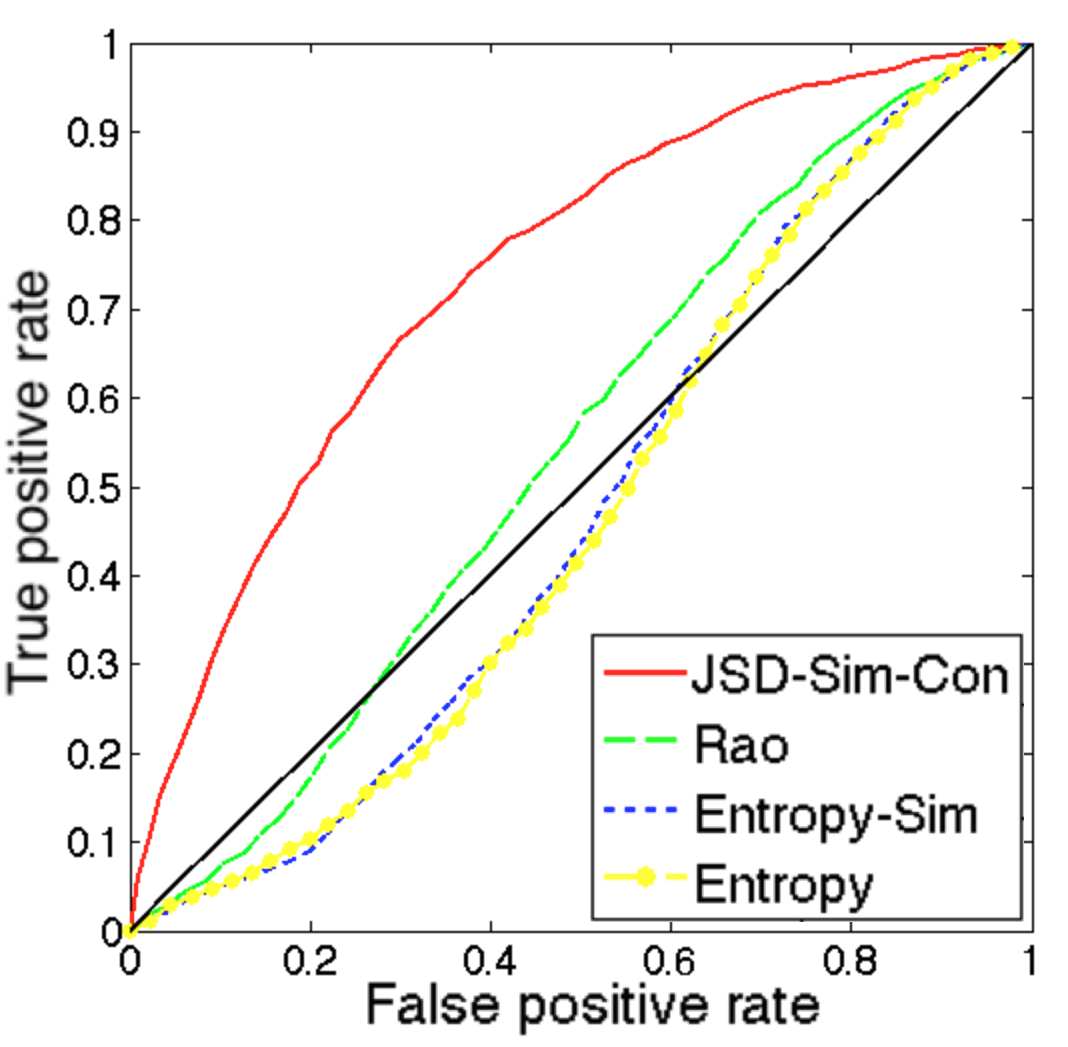
\includegraphics[width=36mm]{figures/phonecases-comparison-kopia.png}
               \caption{eBay (baseline)}
                \label{fig:phonecases-comparison}
        \end{subfigure}%\qquad
              ~ %add desired spacing between images, e. g. ~, \quad, \qquad, \hfill etc.
          %(or a blank line to force the subfigure onto a new line)
        \begin{subfigure}[b]{0.24\textwidth}
                \centering
                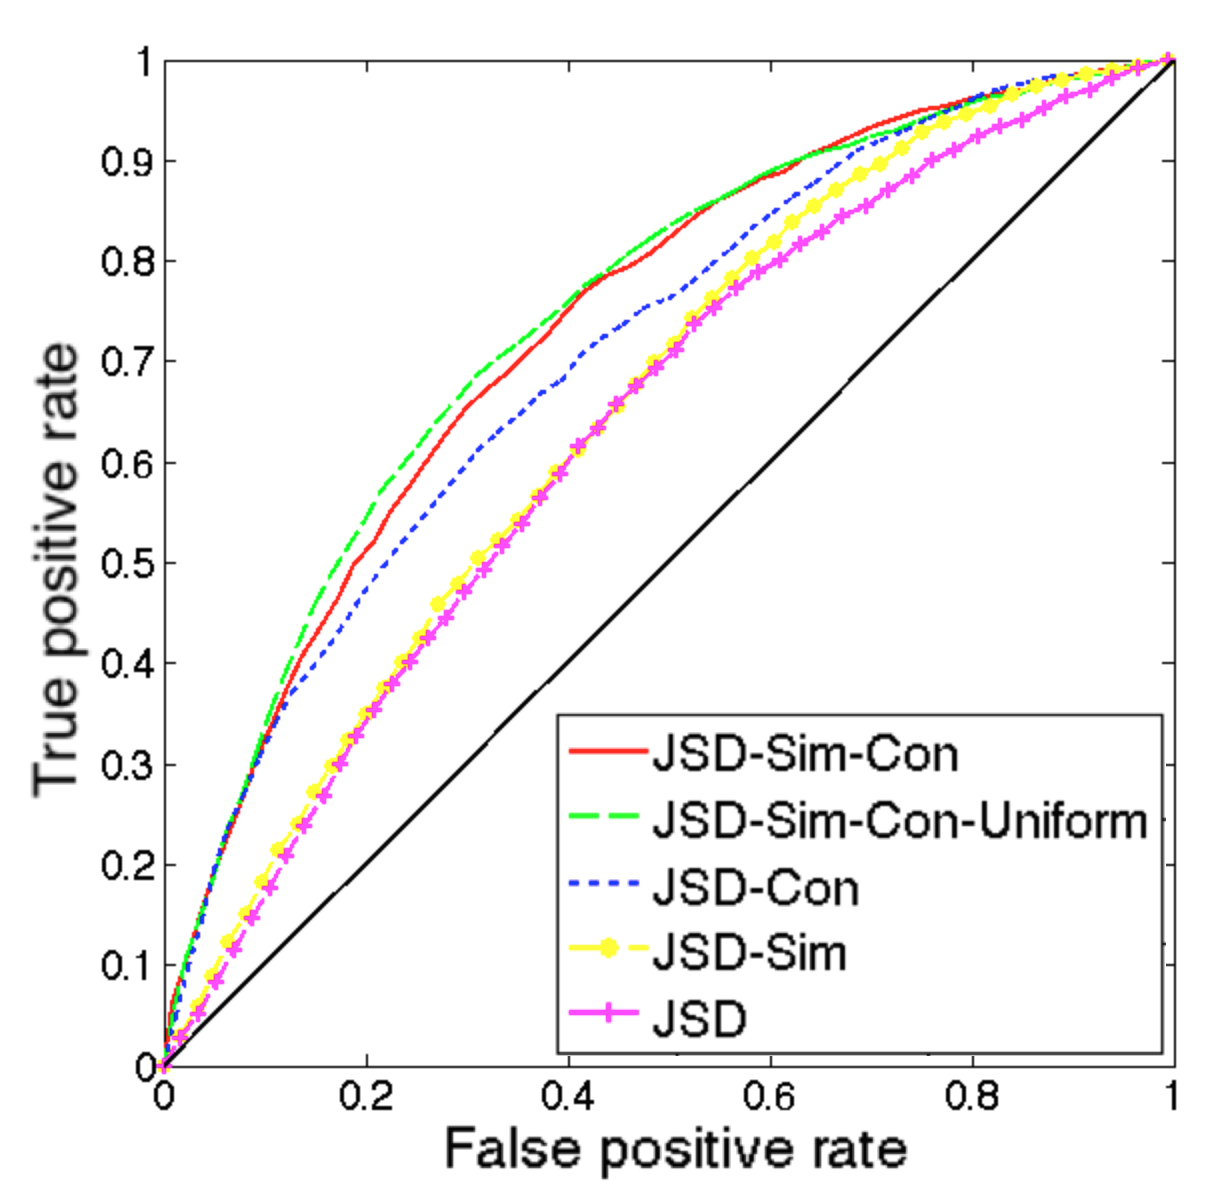
\includegraphics[width=36mm]{figures/phonecases-breakdown-kopia.png}
                \caption{eBay (JSD)}
                \label{fig:phonecases-breakdown}
        \end{subfigure}\nobreak
              ~ %add desired spacing between images, e. g. ~, \quad, \qquad, \hfill etc.
          %(or a blank line to force the subfigure onto a new line)
        \begin{subfigure}[b]{0.24\textwidth}
                \centering
                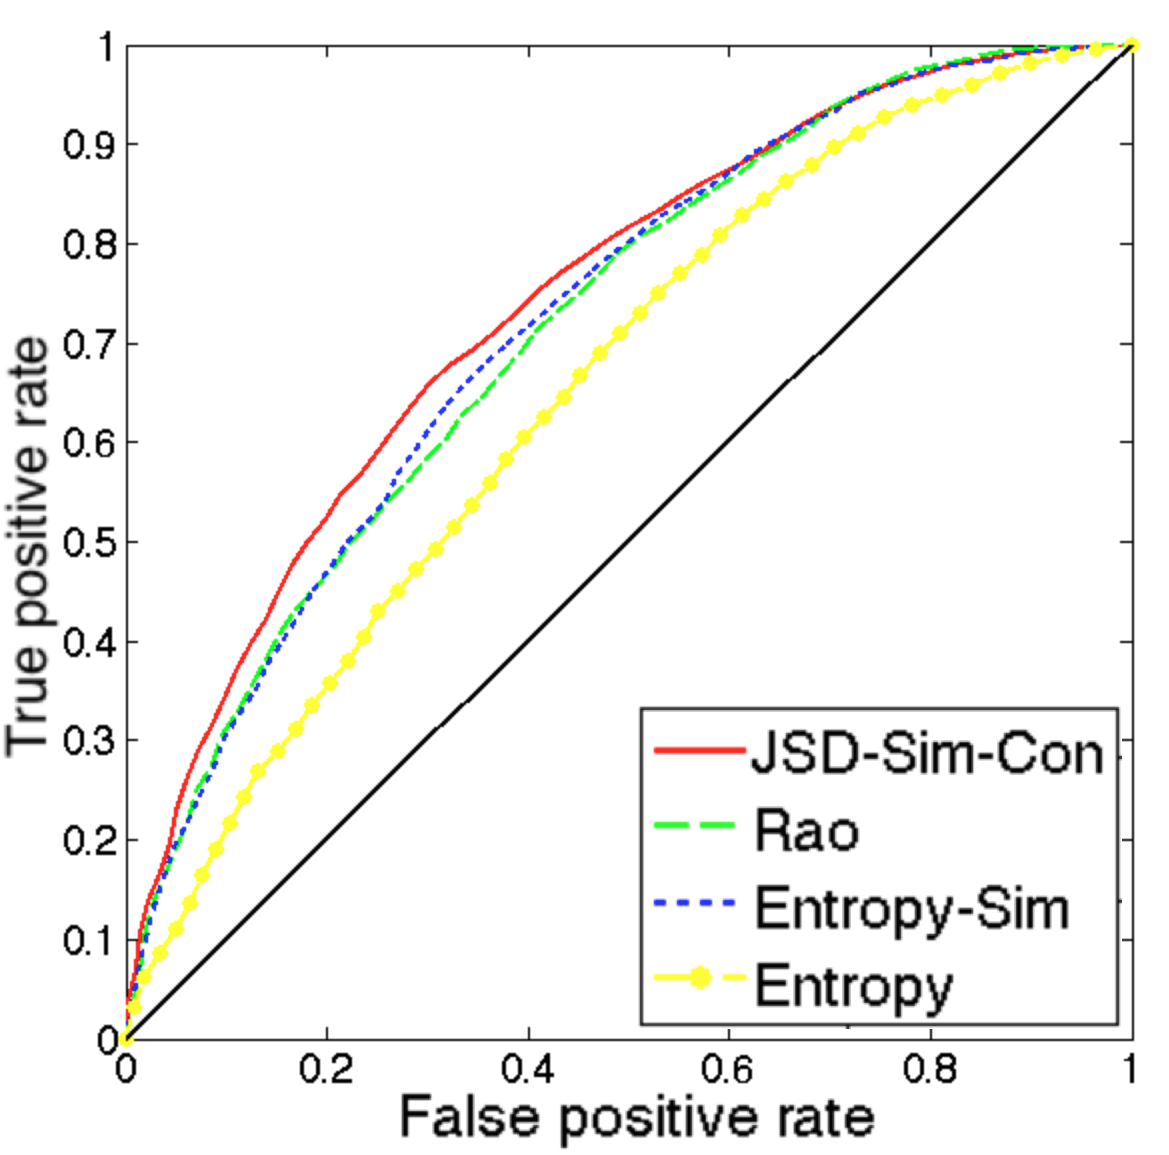
\includegraphics[width=36mm]{figures/nsf-comparison-kopia.png}
                \caption{NSF (baseline)}
                \label{fig:nsf-comparison}
        \end{subfigure}%\qquad
        ~ %add desired spacing between images, e. g. ~, \quad, \qquad, \hfill etc.
          %(or a blank line to force the subfigure onto a new line)
        \begin{subfigure}[b]{0.24\textwidth}
        	        \centering
                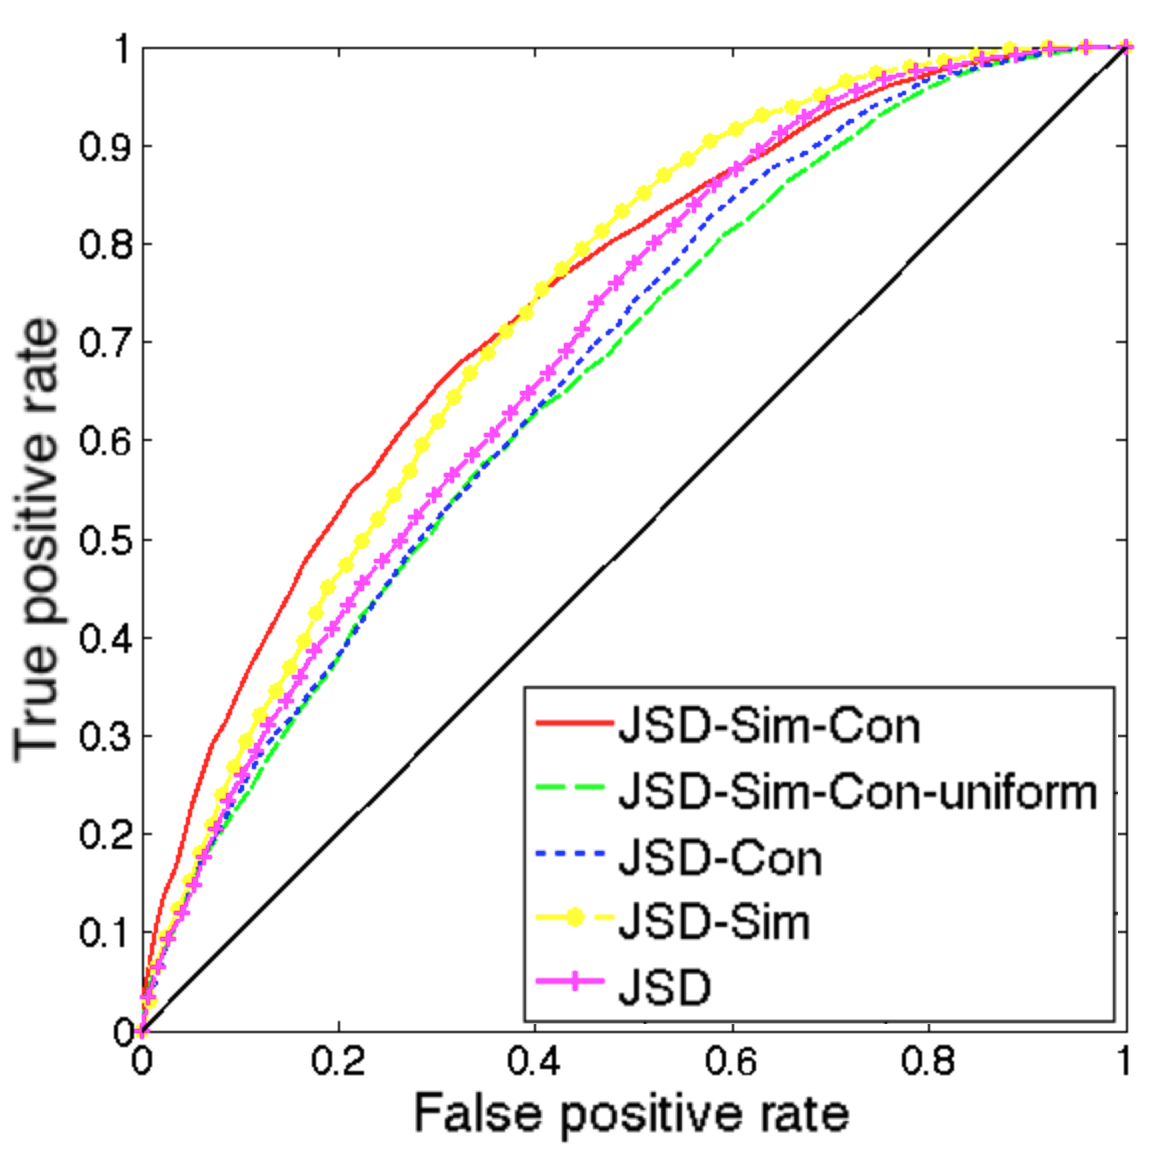
\includegraphics[width=36mm]{figures/nsf-breakdown-kopia.png}
               \caption{NSF (JSD)}
                \label{fig:nsf-breakdown}
        \end{subfigure}
       \caption{ROC curves presenting the results of experiments on
         the eBay dataset (a,b) and NSF proposal dataset (c,d). The
         comparison plots (a,c) show the results for our approach (JSD-Sim-Con)
         against other methods, while the breakdown plots (b,d)
         show different variations of our approach. }\label{fig:roc-curves}
\end{figure}

\begin{comment}
Figure \ref{fig:roc-curves} presents the ROC curves for the
unsupervised task. Analyzing Plot \ref{fig:nsf-comparison} we can see
how our proposed measure (denoted as JSD-Sim-Con) compared to the
baseline methods for the NSF dataset. Note, that in this task the
pieces of text are large enough (a few hundred words on average), to
obtain reasonable topic distributions from Mallet. In particular, this
task is comparable with the one in \cite{bache:2013}. Our measure
obtains the best AUC of approx. $0.74$, however Rao Diversity and
Entropy-Sim both get close to that as well. The regular Entropy
performs significantly worse, which shows that enhancing the topic
distribution with topic-similarities gives significant improvements
even for the Entropic measure of diversity for text. The picture looks
quite different for the eBay dataset, as seen in plot
\ref{fig:phonecases-comparison}. Here, we can see that our measure
still performs very well, with AUC of 0.73, while the other measures
give almost meaningless results. This can be explained easily because
in this set, the text snippets are too short to infer a good topic
distribution directly from the LDA topic model. Plots
\ref{fig:phonecases-breakdown} and \ref{fig:nsf-breakdown}  show how
different versions of our measure perform, and the gains obtained from
each enhancement. Both adding topic-similarity (denoted as {\em Sim})
and context-dependence (denoted as {\em Con})
improves the results, however, their effects are different for each
dataset . Additionally, to find out what is the effect of importance
weights from Definition \ref{importance}, we tested a version of the
measure, which uses uniform weights instead. Interestingly, this had
no negative impact for the eBay dataset, but significantly worsened
the result for the NSF dataset. It appears that, as one would expect,
using importance weights matters more if the analyzed piece of text is
longer.
\end{comment}

\begin{table}[t]
\caption{Classification results for the eBay dataset.}
\label{tab:classification-results}
\vspace{-4mm}
\begin{center}
\begin{tabular}{|l|c|c|c|c|}
\hline
&Precision & Recall & F1 & Accuracy
\\ \hline 
JSD Features         &$\mathbf{0.714}\pm 0.015$&$0.597\pm 0.016$&$0.650\pm
0.014$& $\mathbf{0.8828}\pm 0.0045$\\
RAE             &$0.676\pm 0.005$&$\mathbf{0.666}\pm 0.030$&$\mathbf{0.671}\pm
0.013$&$0.8809\pm 0.0020$ \\
SVD Features             &$0.676\pm 0.008$&$0.633\pm 0.017$&$0.654\pm
0.010$&$0.8778\pm 0.0027$\\
\hline
\end{tabular}
\end{center}
\end{table}

%%%%%%%%%%%%%%%%%%%%%%%%%%%%%%%%%%%%%%%%%%%%%%%%%%%%%%%%%%%%%
%%%%%%%%%%%%%%%%%%%%%%%%%%%%%%%%%%%%%%%%%%%%%%%%%%%%%%%%%%%%%
%%%%%%%%%%%%%%%%%%%%%%%%%%%%%%%%%%%%%%%%%%%%%%%%%%%%%%%%%%%%%

%\section{Conclusions}
%\label{sec:conclusions}

%%%%%%%%%%%%%%%%%%%%%%%%%%%%%%%%%%%%%%%%%%%%%%%%%%%%%%%%%%%%%
%%%%%%%%%%%%%%%%%%%%%%%%%%%%%%%%%%%%%%%%%%%%%%%%%%%%%%%%%%%%%
%%%%%%%%%%%%%%%%%%%%%%%%%%%%%%%%%%%%%%%%%%%%%%%%%%%%%%%%%%%%%




%%%%%%%%%%%%%%%%%%%%%%%%%%%%%%%%%%%%%%%%%%%%%%%%%%%%%%%%%%%%%
%%%%%%%%%%%%%%%%%%%%%%%%%%%%%%%%%%%%%%%%%%%%%%%%%%%%%%%%%%%%%
%%%%%%%%%%%%%%%%%%%%%%%%%%%%%%%%%%%%%%%%%%%%%%%%%%%%%%%%%%%%%

\bibliographystyle{plain}
\bibliography{nips2014}


\end{document}
